% Русская версия отчёта H1 (XeLaTeX)
\documentclass[11pt,a4paper]{article}
\usepackage{fontspec}
\setmainfont{cmunrm}[Extension=.otf,BoldFont=cmunbx,ItalicFont=cmunti,BoldItalicFont=cmunbi]
\setsansfont{cmunss}[Extension=.otf,BoldFont=cmunsx,ItalicFont=cmunsi,BoldItalicFont=cmunso]
\setmonofont{cmuntt}[Extension=.otf,BoldFont=cmuntb,ItalicFont=cmunit,BoldItalicFont=cmuntx]
\usepackage[english,russian]{babel}
\usepackage[margin=2.2cm]{geometry}
\usepackage{amsmath,amssymb,amsthm,mathtools,bm}
\usepackage{graphicx,booktabs,tabularx,xltabular,array,multirow,enumitem,xcolor}
\usepackage[most]{tcolorbox}
\usepackage{tikz}
\usetikzlibrary{arrows.meta,positioning,shapes.geometric,fit}
\usepackage[colorlinks,linkcolor=blue!50!black,citecolor=green!35!black,urlcolor=blue!50!black]{hyperref}
\setlist{itemsep=1pt,topsep=2pt}
\setlength{\emergencystretch}{3em}
\numberwithin{equation}{section}

\newtheorem{theorem}{Теорема}[section]
\newtheorem{lemma}[theorem]{Лемма}
\newtheorem{proposition}[theorem]{Предложение}
\newtheorem{corollary}[theorem]{Следствие}
\theoremstyle{definition}
\newtheorem{definition}[theorem]{Определение}
\newtheorem{assumption}[theorem]{Предположение}
\theoremstyle{remark}
\newtheorem{remark}[theorem]{Замечание}
\newtheorem{example}[theorem]{Пример}

\newcommand{\E}{\mathbb E}\newcommand{\R}{\mathbb R}\newcommand{\N}{\mathbb N}\let\Prob\relax\newcommand{\Prob}{\mathbb P}
\newcommand{\norm}[1]{\lVert #1\rVert}\newcommand{\abs}[1]{\lvert #1\rvert}\newcommand{\ip}[2]{\langle #1,#2\rangle}
\newcommand{\Dmax}{\Delta_{\max}}\newcommand{\Dcp}{\Delta_{\rm cp}}
\newcommand{\cN}{\mathcal N}\newcommand{\cG}{\mathcal G}\newcommand{\cF}{\mathcal F}\newcommand{\cS}{\mathcal S}
\newcommand{\Unif}{\mathrm{Unif}}\newcommand{\TV}{\mathrm{TV}}\newcommand{\tmix}{t_{\rm mix}}
\newcommand{\Sph}{\mathbb S^{d-1}}\newcommand{\Ball}{\mathbb B}
\newcommand{\hatm}{\hat m_\gamma}\newcommand{\supp}{\operatorname{supp}}
\newcommand{\status}[1]{\textsf{\small[#1]}}
\newcommand{\ok}{\textcolor{green!45!black}{\textsf{доказано}}}
\definecolor{hl}{HTML}{2a78d6}
\tcbset{card/.style={colback=blue!2,colframe=blue!45!black,boxrule=0.6pt,arc=2pt,left=6pt,right=6pt,top=4pt,bottom=4pt,fonttitle=\bfseries}}

\title{\textbf{H1: структура класса $\cN(\Delta,\tau,\gamma)$\\ и корректное определение $\Dmax$}\\[2pt]
\large Отчёт о локальном исследовании}
\author{}
\date{11~ноября 2026~г.}

\begin{document}
\maketitle

\tableofcontents

%=====================================================================================================
\setcounter{section}{-1}
\section{Карточка-резюме}\label{sec:card}
\begin{tcolorbox}[card,title={H1 на одной странице}]
\textbf{Гипотеза.} Условие (2) ограничивает только $m=\E_\pi\delta$; при фиксированном $\gamma$ класс содержит нетривиальные «бесселевы» $m$,
а при всех $\gamma\le\gamma_0$ оно влечёт $m\equiv\mathrm{const}$; без фиксированного бюджета $\Dmax=\infty$, поэтому $T$ и протокол запросов должны входить в определение.

\textbf{Вердикт: подтверждена в уточнённой форме.} Четыре математических утверждения доказаны (для ограниченного измеримого шума, при прочтении условия (2)
для почти всех $x$), алгоритмические~--- при условиях, указанных ниже и в~\S\ref{sec:verdict} ($\gamma\le\varepsilon/(4M)$ для класса с фиксированным радиусом; вариант «в среднем», а для варианта «по вероятности»~--- с заменой $\varepsilon\to\beta\varepsilon$); два уточнения: (i)~\emph{двух радиусов} $\gamma_1,\gamma_2$ с $\gamma_1/\gamma_2\notin\{j_{d/2,k}/j_{d/2,l}\}$ уже достаточно, чтобы $m\equiv{\rm const}$ (доказано на $\R^d$; на шаре только процитировано), но в высокой размерности второй радиус $\gamma_2\gtrsim\gamma_1$ количественно почти бесполезен;
(ii)~протокол важен: если холостые раунды бесплатны, $\tau$ полностью выпадает из задачи (предл.~\ref{prop:wait}).

\textbf{Главный результат (одна формула).} При пакетировании по состояниям (batching) и прогреве (burn-in) длиной $t_0=\tau\lceil\log_2(16R\sqrt d\,\Delta/(\gamma\varepsilon))\rceil_+$ раундов $\E f(\bar x)-f^*\le\varepsilon$ после
\[
T(\Delta)=\Big\lceil\tfrac{145}{4}\tfrac{M^2R^2}{\varepsilon^2}\Big\rceil\Big(\Big\lceil \tfrac{2d^2}{d-1}+(2d+8\tau-3)\,\tfrac{d\Delta^2}{M^2\gamma^2}\Big\rceil+t_0\Big)
=O\!\Big(\tfrac{R^2}{\varepsilon^2}\big[dM^2+(d+\tau)\tfrac{d\Delta^2}{\gamma^2}\big]+\tau\log\Big)
\]
раундов для любого $\Delta<\infty$ при условии $\gamma\le\varepsilon/(4M)$ (теор.~\ref{thm:alg}; вариант «в среднем»). Следовательно, без бюджета $\Dmax=\infty$ \emph{для класса всех радиусов} (безусловно: там $\E_\pi\delta={\rm const}$, и алгоритм сам выбирает радиус) \emph{и для класса с фиксированным радиусом при $\gamma\le\varepsilon/(4M)$}; для класса с фиксированным радиусом при $\gamma>\varepsilon/(4M)$ ничего не доказано (H6). Далее,
$\Dmax^{\E}(T)\ \ge\ \frac{\varepsilon\gamma}{R}\sqrt{T/\big(74.5\,(2d+8\tau-3)\,d\big)}$ при $\gamma\le\varepsilon/(4M)$ и $T\ge 2T_1(\Delta)$, так что $T\gtrsim\tau(MR/\varepsilon)^2\log$,~--- это \emph{первая ветвь} нижней половины H2, доказанная вне режима $\tau\gtrsim T$. В варианте «по вероятности» опр.~\ref{def:dmax} то же верно с заменой $\varepsilon\to\beta\varepsilon$ (неравенство Маркова, следствие~\ref{cor:prob}).

\textbf{Что это означает для задачи.} Без бюджета порог вырожден, поэтому невырожденный $\Dmax$ содержит бюджет раундов $T$ и протокол с $q$ запросами (один шаг цепи за раунд, холостые раунды учитываются, экзогенная цепь), а «ожидаемая картина»~--- это утверждение об \emph{уровне, сохраняющем сложность}, $\Dcp(C)=\Dmax(T=C\,T_0)$. В варианте «в среднем» $\Dcp(C)\ge M\gamma/\sqrt{2d+8\tau-3}$ при $\gamma\le\varepsilon/(4M)$ и $C\ge\frac{149}4(6+t_0/d)$ (например, $C=261$, если $\tau\lceil\log_2(16MR/\varepsilon)\rceil\le d$); это нижняя сторона «ожидаемой картины» $M\gamma/\sqrt d$, и здесь доказана только нижняя сторона (опр.~\ref{def:dmax}, следствие~\ref{cor:cp}). В классе всех радиусов условие (2) для всех $\gamma\le\gamma_0$ сводится к условию «$\E_\pi\delta(x,\cdot)={\rm const}$» (теор.~\ref{thm:allgamma}); там $\gamma$ выходит из определения класса и становится параметром алгоритма.

\textbf{Численные эксперименты.} E1.1, E1.3, E1.4 (по 5~зёрен генератора (seeds) каждый) согласуются со своими предсказаниями: нули Бесселя дают смещение на уровне погрешности Монте-Карло (МК), смещение вне нулей совпадает с $\Delta t\Psi_d(t)/d$; настроенная волна при втором радиусе следует $\Delta|\omega||\Psi_d(\gamma_2|\omega|)|$; второй момент пакетной оценки совпадает с точным значением $A+S\,(1+\alpha)/(1-\alpha)$ с точностью до $1.41\%$ (аддитивен по $d$ и $\tau$). E1.2 (логистическая регрессия): цель достигается при каждом $\Delta$, и бюджет согласуется с $\Delta^2$~--- точечная оценка наклона $2.31$ на $0.01$ выше заранее зафиксированного диапазона $2\pm0.3$, тогда как её ДИ $[1.97,2.65]$ и тест совмещения (collapse) содержат $2$ (\S\ref{sec:num}).

\end{tcolorbox}

%=====================================================================================================
\section{Место в глобальной задаче}\label{sec:place}
\textbf{Закрываемые узкие места.} H1 относится к двум узким местам постановки задачи:
(i)~определение $\Dmax$ не фиксирует ни бюджет, ни протокол запросов, а при «полиномиальном числе вызовов» центрированный шум усредняется при любом уровне;
(ii)~роль $\gamma$ в классе (фиксированный радиус или все радиусы $\le\gamma_0$) не определена.
Все остальные гипотезы сформулированы в терминах $\Dmax$, поэтому H1 предшествует им всем.

\begin{figure}[h]
\centering
\begin{tikzpicture}[node distance=7mm and 9mm, every node/.style={font=\small},
  h/.style={draw,rounded corners=2pt,minimum width=12mm,minimum height=6mm,fill=gray!6},
  cur/.style={h,fill=hl!18,draw=hl,line width=1.1pt},
  ar/.style={-{Stealth[length=2mm]},gray!70!black}, dar/.style={ar,dashed}]
\node[cur] (H1) {\textbf{H1} определение};
\node[h,below left=9mm and 22mm of H1] (H3) {H3 $\tau{=}1$};
\node[h,right=6mm of H3] (H4) {H4 редукция};
\node[h,right=6mm of H4] (H5) {H5 трудн.\ констр.};
\node[h,right=6mm of H5] (H6) {H6 $\gamma$-переход};
\node[h,below=12mm of H4] (H2) {\textbf{H2} $\Dmax(T,\tau)$};
\node[h,right=14mm of H2] (H9) {H9 $T_{\rm eff}$};
\node[h,left=14mm of H2] (H8) {H8 ленивая цепь};
\node[h,below=8mm of H8] (H7) {H7 самодизеринг};
\node[h,below=8mm of H2] (H10) {H10 общий дизеринг};
\draw[ar,line width=1pt,hl] (H1) -- (H3); \draw[ar,line width=1pt,hl] (H1) -- (H4);
\draw[ar,line width=1pt,hl] (H1) -- (H5); \draw[ar,line width=1pt,hl] (H1) -- (H6);
\draw[ar,line width=1pt,hl] (H1.west) to[out=190,in=110] (H8.north);
\draw[ar] (H3) -- (H2); \draw[ar] (H4) -- (H2); \draw[ar] (H5) -- (H2);
\draw[ar] (H2) -- (H8); \draw[ar] (H2) -- (H9); \draw[ar] (H7) -- (H8); \draw[dar] (H2) -- (H10); \draw[dar] (H6) -- (H2);
\node[font=\scriptsize,text=hl,align=left,right=3mm of H1] {первая ветвь нижней половины H2\\доказана здесь при $T\gtrsim\tau(MR/\varepsilon)^2\log$\\(следствие~\ref{cor:lower}); протокол с экзогенной\\цепью зафиксирован для H8};
\end{tikzpicture}
\caption{Зависимости между H1--H10 (стрелки: «используется в»). H1 (выделена) даёт определение, которым пользуются все остальные; H3/H4 дают нижнюю сторону H2, H3/H5~--- верхнюю; ветвь округления (H7, H8, H10) берёт из H2 точку перехода $\tau\approx T$.}
\label{fig:diagram}
\end{figure}

\textbf{Зависит от:} ничего (H1~--- корень). \textbf{Используется в:} H2--H6 (определение, сведение класса к $m$ и $\xi$), H8 (протокол: цепь здесь экзогенная, цепь, порождённая методом, исключена и должна рассматриваться отдельно), H9 (доказательство ниже использует только равномерное перемешивание, которое H9 стремится ослабить).

%=====================================================================================================
\section{Постановка и мотивация}\label{sec:statement}
\subsection{Постановка и обозначения}
$\Ball=\{u\in\R^d:\norm u\le1\}$, $\Sph=\partial\Ball$, $e\sim\Unif(\Sph)$, $u\sim\Unif(\Ball)$, $B_r=r\Ball$; $d\ge2$.
Для $g\in L^\infty(\R^d)$ сглаживание по шару равно $\hat g_\gamma(x)=\E_u g(x+\gamma u)=(g*\chi_\gamma)(x)$, $\chi_\gamma=\abs{B_\gamma}^{-1}\mathbf 1_{B_\gamma}$.
Мультипликаторы шара и сферы:
\begin{equation}\label{eq:Psi}
\Psi_d(t)=\E_u e^{\mathrm i t u_1}=\Gamma(\tfrac d2+1)\big(\tfrac2t\big)^{d/2}J_{d/2}(t),\qquad
\Phi_d(t)=\E_e e^{\mathrm i t e_1}=\Gamma(\tfrac d2)\big(\tfrac2t\big)^{d/2-1}J_{d/2-1}(t),
\end{equation}
$\Psi_d(0)=\Phi_d(0)=1$; $j_{\nu,k}$~--- $k$-й положительный нуль $J_\nu$. Преобразование Фурье: $\hat u(\xi)=\int u(x)e^{-\mathrm i\ip\xi x}dx$ на $\cS'(\R^d)$.

\textbf{Оракул.} $O(x,s)=f(x)+\delta(x,s)$, $f$ выпукла и $M$-липшицева на $B_R$; $(s_k)$~--- марковская цепь на стандартном борелевском пространстве $(S,\mathcal S)$ с ядром $P$, стационарным распределением $\pi$,
$d(t)=\sup_{s}\norm{P^t(s,\cdot)-\pi}_\TV$ и временем перемешивания $\tau=\tmix=\min\{t\ge1:d(t)\le\frac14\}$.
$\delta:\R^d\times S\to[-\Delta,\Delta]$ совместно борелевская. Условие класса из постановки задачи:
\begin{equation}\label{eq:orth}
\E_{s\sim\pi}\E_e\big[\delta(x+\gamma e,s)\,e\big]=0\qquad\forall x. \tag{2}
\end{equation}
\textbf{Разложение.} $m(x)=\E_\pi\delta(x,\cdot)$, $\xi=\delta-m$ (так что $\abs m\le\Delta$, $\abs\xi\le2\Delta$, $\E_\pi\xi(x,\cdot)=0$ для каждого $x$).
\textbf{Смещение при фиксированном состоянии} (двухточечная оценка $\hat g=\frac d{2\gamma}(O(x+\gamma e,s)-O(x-\gamma e,s))e$):
$b(x,s)=\frac d{2\gamma}\E_e[(\delta(x+\gamma e,s)-\delta(x-\gamma e,s))e]=\frac d\gamma\E_e[\delta(x+\gamma e,s)e]$ в силу замены $e\mapsto-e$.

\textbf{Два прочтения (2)} для ограниченной измеримой $\delta$: (A)~для почти всех (по Лебегу) $x$; (B)~для каждого $x$.
\textbf{Регулярный класс} $\cG_\gamma$: ограниченные борелевские $g$, такие что для каждого $x$ множество $\{\theta\in\Sph:\ g$ разрывна в точке $x+\gamma\theta\}$ имеет поверхностную меру $0$.
Примеры: непрерывные $g$; $g$, разрывы которых лежат на счётном числе аффинных гиперплоскостей (хэш-шум по ячейкам сетки, шум $\mathrm{sign}\sin\ip vx$, округление функции, аффинной на шаблоне (stencil)), поскольку гиперплоскость пересекает сферу по множеству меры нуль.

\subsection{Утверждения}
\begin{center}\small
\begin{tabularx}{\textwidth}{@{}lX@{}}
\toprule
H1.1 & $\frac d\gamma\E_e[\delta(x+\gamma e,s)e]=\nabla_x\hat\delta_\gamma(x,s)$ для почти всех $x$ (для каждого $x$ в $\cG_\gamma$); $\E_\pi$ и $\E_e$ перестановочны; (2) $\iff\hat m_\gamma\equiv{\rm const}$; выбор (A)/(B) не меняет ни одного результата. \\
H1.2 & При фиксированном $\gamma$ функция $\Delta\cos(\ip\omega x+\varphi)$ лежит в классе тогда и только тогда, когда $\gamma|\omega|\in\{j_{d/2,k}\}$; все допустимые $m\in L^\infty$: $\widehat{m-c}$~--- простой слой на сферах $|\xi|=j_{d/2,k}/\gamma$. \\
H1.3 & (2) для всех $\gamma\in(0,\gamma_0]$ $\Rightarrow m\equiv c$; сильнее: достаточно двух радиусов с $\gamma_1/\gamma_2\notin Q_d=\{j_{d/2,k}/j_{d/2,l}\}$; результат точен. \\
H1.4 & Без бюджета $\Dmax=\infty$: явный алгоритм с $\E\hat g=\nabla f_\gamma$ (с точностью до сколь угодно малого смещения), вторым моментом $\lesssim dM^2+(d+\tau)d\Delta^2/\gamma^2$ и явным $N(\Delta,\varepsilon,d,\tau)=O(\Delta^2)$. \\
H1.5 & Варианты протокола и их влияние на $\Dmax$; ожидаемая картина описывает уровень, сохраняющий сложность, $\Dcp=\Dmax(C\,T_0)$. \\
\bottomrule
\end{tabularx}
\end{center}

\subsection{Почему это стоит проверять; следствия}
Если H1 верна, то двусторонние оценки, которых требует постановка задачи, являются оценками \emph{функции бюджета} $T$; число $M\gamma/\sqrt d$~--- это уровень, до которого шум не меняет порядок сложности, а не граница разрешимости.
Тогда класс чисто расщепляется: $m$~--- детерминированная, настроенная на радиус часть, невидимая на радиусе метода; $\xi$~--- центрированная марковская часть, которая обходится только дисперсией.
Если бы H1 была неверна (например, если бы некоторый ограниченный центрированный шум делал $\varepsilon$ недостижимым при любом бюджете), то задача в нынешней постановке уже имела бы конечный ответ, а ожидаемая картина была бы границей разрешимости. Тогда буквальная формулировка («полиномиальное число вызовов») имела бы смысл.

%=====================================================================================================
\section{Что известно}\label{sec:known}
{\small
\begin{xltabular}{\textwidth}{@{}p{3.3cm}Xp{2.6cm}@{}}
\toprule
\textbf{Пункт} & \textbf{Утверждение в том виде, в каком оно используется} & \textbf{Статус здесь}\\\midrule
\endhead
Градиент сглаживания по шару & $\nabla\hat f_\gamma(x)=\frac d\gamma\E_e[f(x+\gamma e)e]$; Flaxman, Kalai, McMahan (SODA 2005), лемма~1, для интегрируемых $f$ через формулу Стокса; обзор Gasnikov et al.\ arXiv:2211.13566, \S4.4 для условия (2) (номер теоремы в обзоре не перепроверен). & передоказано для $L^\infty$ с различением «почти всюду / всюду» (лемма~\ref{lem:stokes}) \\
Второй момент двухточечной оценки & $\E\norm{\hat g}^2\le c\,dM^2$, Shamir (JMLR 18, 2017), через концентрацию на сфере. & выведено заново с $c=d/(d-1)$ через неравенство Пуанкаре на $\Sph$ (лемма~\ref{lem:var}) \\
MALN & Pasechnyuk-Vilensky, Pavlov, Takáč, Gasnikov, arXiv:2306.16371\textbf{v5}: опр.~II.1 (оракул $O_\delta(f)$, $T$ запросов в $B_R$, рандомизированный адаптивный алгоритм), опр.~II.2 ($(\varepsilon,\beta,\delta,T)$-разрешимость, $\Delta_\cF(\varepsilon,\beta,T)=\sup\{\delta\}$), теор.~III.1 ($\Delta\le\frac43\varepsilon\theta^2+\frac53\frac{\varepsilon^2\theta}{MR}$, $\theta_*=\sqrt{2\ell/(n-1)}$, $\ell=\log\frac{2(T+1)}{1-\beta}$), предл.~IV.1 (двухточечный метод выдерживает $\varepsilon^2/(84\sqrt nMR)$ при бюджетах $T\ge J(2K+1)$, $K=\lceil1200\,n^2M^2R^2/\varepsilon^2\rceil$, $J$ определено там же), следствие~IV.4. Шум там~--- фиксированное детерминированное возмущение $f$. & использовано как образец для опр.~\ref{def:dmax}; не передоказано \\
Помпейю / периодические в среднем функции & Schwartz (Ann.\ Math.\ 48, 1947): спектральный синтез для периодических в среднем функций на $\R$. Brown, Schreiber, Taylor (Ann.\ Inst.\ Fourier 23(3), 1973, 125--154): теор.~3.1/3.4~--- замкнутые подпространства $C(\R^2)$, инвариантные относительно сдвигов и вращений (замечание: $\R^n$), порождаются содержащимися в них экспоненциальными многочленами; теор.~4.4~--- два круга радиусов $r_1,r_2$ обладают свойством Помпейю тогда и только тогда, когда $r_1/r_2\notin Q_1(0)$, счётного множества, определяемого нулями Бесселя (эта теорема Помпейю о двух кругах доказана также у Zalcman, Arch.\ Rational Mech.\ Anal.\ 47, 1972, 237--254); теор.~4.7~--- вариант теоремы Дельсарта о двух радиусах для \emph{гармоничности} с мерой площади, взятый из Zalcman [19] (другое утверждение, здесь не используется). Общее $d$ и локальные варианты: Berenstein--Zalcman (1976, 1980), Berenstein--Gay (Israel J.\ Math.\ 1986, $d=2$, требуется $R>r_1+r_2$), Volchkov, \emph{Integral Geometry and Convolution Equations} (Kluwer 2003). & глобальные утверждения передоказаны для ограниченных $m$ рассуждением с обобщёнными функциями умеренного роста (теор.~\ref{thm:fourier}, \ref{thm:tworadii}); ссылки на локальные варианты и общее $d$ \textbf{не перепроверены} \\
Структура обобщённых функций на подмногообразии & Hörmander, \emph{ALPDO I}, теор.~2.3.5: обобщённая функция с носителем в $\{x''=0\}$ локально имеет вид $\sum_{|\alpha|\le k}u_\alpha\otimes\delta^{(\alpha)}(x'')$. & используется \\
Перемешивание & $\bar d(s+t)\le\bar d(s)\bar d(t)$, $d\le\bar d\le2d$ $\Rightarrow d(\ell\tmix)\le2^{-\ell}$ (Levin--Peres--Wilmer, \emph{Markov Chains and Mixing Times}, гл.~4). & используется; проверено численно (V6) \\
Марковские методы нулевого порядка & Prokhorov, Chebykin, Gasnikov, Beznosikov, arXiv:2601.01160: для безградиентных методов с марковским шумом цена корреляции аддитивна, $d+\tau$. & в доказательствах не используется; согласуется с леммой~\ref{lem:var} \\
\midrule
Получено ранее в этом проекте & Пилотный расчёт Монте-Карло, выполненный до этого исследования: $d=5$, $\gamma|\omega|=5.763$ даёт $2.3\cdot10^{-4}$ при погрешности МК $2.2\cdot10^{-4}$. Округление с равномерным сдвигом $c$ удовлетворяет (2) для всех радиусов при равномерном законе сдвига: $\E_c\delta(x,c)$~--- среднее «пилы» округления за один период, константа, не зависящая от $x$. & пилотный расчёт: как таковой не перепроверен (его значение воспроизведено в E1.1); округление: непосредственное рассуждение \\
\midrule
Новое в этом отчёте & Лемма~\ref{lem:stokes}--следствие~\ref{cor:cp}, предл.~\ref{prop:wait}, предл.~\ref{prop:q1}, предл.~\ref{prop:quant}; эксперименты E1.1--E1.4; проверки V1--V10, S1--S7. & \\
\bottomrule
\end{xltabular}}

%=====================================================================================================
\section{Теория}\label{sec:theory}
\subsection{H1.1: смещение при фиксированном состоянии, два прочтения и сведение к $m$}

\begin{lemma}[Измеримость и перестановка]\label{lem:fubini}
Пусть $\delta:\R^d\times S\to[-\Delta,\Delta]$ измерима относительно $\mathcal B(\R^d)\otimes\mathcal S$. Тогда $m=\E_\pi\delta(\cdot,s)$ борелевская, $\abs m\le\Delta$, и для \emph{каждого} $x$ и $\gamma>0$
\[\E_{s\sim\pi}\E_e[\delta(x+\gamma e,s)e]=\E_e\E_{s\sim\pi}[\delta(x+\gamma e,s)e]=\E_e[m(x+\gamma e)e].\]
\end{lemma}
\begin{proof}
Отображение $(\theta,s)\mapsto\delta(x+\gamma\theta,s)\theta_i$ измеримо на $\Sph\times S$ и ограничено величиной $\Delta$, а значит, интегрируемо по $\sigma\otimes\pi$; теорема Фубини--Тонелли даёт и равенство повторных интегралов, и измеримость $m$.
\end{proof}
\begin{remark}
От совместной измеримости нельзя отказаться: для подынтегральных функций, измеримых по каждой переменной, но не совместно, два повторных интеграла могут различаться (примеры типа Серпинского). Это естественное предположение: $\delta$~--- функция от $(x,s)$, вычисляемая оракулом.
\end{remark}

\emph{Почему лемма~\ref{lem:stokes} должна быть верна и в чём трудность.} Для гладких $g$ тождество есть теорема о дивергенции на шаре. Для $g\in L^\infty$ правая часть~--- поверхностный интеграл по сфере $x+\gamma\Sph$, множеству лебеговой меры нуль, так что она зависит от выбора представителя $g$, а левая часть не зависит. Разрешение: сферическое среднее определено для каждого $x$ при заданной борелевской функции, но внутренний смысл имеет только его класс почти всюду.

\begin{lemma}[Формула Стокса на шаре для ограниченных функций]\label{lem:stokes}
Пусть $g$ ограничена и борелевская, $\gamma>0$, $S_g(x)=\frac d\gamma\E_e[g(x+\gamma e)e]$ (определено для каждого $x$).
\begin{enumerate}[label=(\alph*)]
\item $\hat g_\gamma$ липшицева с константой $\sqrt d\norm g_\infty/\gamma$ и $\nabla\hat g_\gamma=S_g$ почти всюду. Если $g=g'$ почти всюду, то $S_g=S_{g'}$ почти всюду.
\item Если $g\in\cG_\gamma$, то $S_g$ непрерывна, $\hat g_\gamma\in C^1$ и $\nabla\hat g_\gamma(x)=S_g(x)$ для каждого $x$.
\item Без (b) тождество может нарушаться в отдельных точках: для $g(y)=\mathbf 1\{\norm y=\gamma\}\,\mathrm{sign}\,y_1$ имеем $\hat g_\gamma\equiv0$, но $S_g(0)=\frac d\gamma\E\abs{e_1}\,\mathbf e_1\ne0$.
\end{enumerate}
\end{lemma}
\begin{proof}
(a) \emph{Гладкий случай.} Если $g\in C^1_b$, то $\partial_i\hat g_\gamma(x)=\abs{B_\gamma}^{-1}\int_{B_\gamma}\partial_ig(x+z)dz=\abs{B_\gamma}^{-1}\int_{\partial B_\gamma}g(x+z)\frac{z_i}\gamma dS(z)$ по теореме о дивергенции, и при $\abs{\partial B_\gamma}=\gamma^{d-1}d\abs{\Ball}$, $\abs{B_\gamma}=\gamma^d\abs\Ball$ это есть $(S_g)_i(x)$.
\emph{Оценка.} Для единичного $v$: $\abs{\ip{S_g(x)}v}\le\frac d\gamma\norm g_\infty\E\abs{\ip ev}\le\frac d\gamma\norm g_\infty(\E\ip ev^2)^{1/2}=\frac{\sqrt d}\gamma\norm g_\infty$.
\emph{Общий случай.} Пусть $g_k=g*\varphi_k$ со стандартным сглаживающим ядром (mollifier); $\norm{g_k}_\infty\le\norm g_\infty$, $g_k\to g$ почти всюду и в $L^1_{\rm loc}$. Тогда $\hat g_{k,\gamma}\to\hat g_\gamma$ поточечно (теорема о мажорируемой сходимости), и каждая $\hat g_{k,\gamma}$ является $\sqrt d\norm g_\infty/\gamma$-липшицевой, значит, такова и $\hat g_\gamma$. Для компакта $K$
$\int_K\norm{S_{g_k}-S_g}dx\le\frac d\gamma\int_{\Sph}\int_K\abs{g_k(x+\gamma\theta)-g(x+\gamma\theta)}dx\,d\sigma(\theta)\to0$, так что $S_{g_k}\to S_g$ в $L^1_{\rm loc}$. Для пробной функции $\phi$:
$\int\hat g_\gamma\partial_i\phi=\lim\int\hat g_{k,\gamma}\partial_i\phi=-\lim\int(S_{g_k})_i\phi=-\int(S_g)_i\phi$. Липшицева функция дифференцируема почти всюду (теорема Радемахера), и её градиент почти всюду совпадает с обобщённым градиентом; следовательно, $\nabla\hat g_\gamma=S_g$ почти всюду.
Если $g=g'$ вне множества меры нуль $N$ (без ограничения общности борелевского), то $\int_{\R^d}\sigma\{\theta:x+\gamma\theta\in N\}dx=\int_{\Sph}\abs{N-\gamma\theta}d\sigma=0$, так что $S_g=S_{g'}$ для почти всех $x$.

(b) Если $x_n\to x$, то $g(x_n+\gamma\theta)\to g(x+\gamma\theta)$ для $\sigma$-почти всех $\theta$ (исключительные $\theta$~--- те, при которых $g$ разрывна в точке $x+\gamma\theta$), так что $S_g(x_n)\to S_g(x)$ по теореме о мажорируемой сходимости. Для липшицевой $u$ с $\nabla u=S$ почти всюду и непрерывной $S$ равенство $u(x+h)-u(x)=\int_0^1\ip{S(x+th)}h\,dt$ выполнено для почти всех $x$ (теорема Фубини вдоль прямых), и обе части непрерывны по $x$, поэтому оно выполнено для всех $x$; значит, $u\in C^1$ и $\nabla u=S$.

(c) $g\ne0$ только на сфере $\partial B_\gamma$, множестве меры нуль, поэтому $\hat g_\gamma\equiv0$; при $x=0$ каждая точка $\gamma e$ лежит на этой сфере и $S_g(0)=\frac d\gamma\E[\mathrm{sign}(e_1)e]=\frac d\gamma\E\abs{e_1}\mathbf e_1$. При $x\ne0$ сфера $x+\gamma\Sph$ пересекает $\partial B_\gamma$ по множеству меры нуль и $S_g(x)=0$. (Проверено численно: V7.)
\end{proof}

\begin{proposition}[Сведение к $m$]\label{prop:reduction}
В условиях леммы~\ref{lem:fubini}:
\begin{enumerate}[label=(\alph*)]
\item $b(x,s)=\nabla_x\hat\delta_\gamma(x,s)$ для почти всех $x$ (для каждого $x$, если $\delta(\cdot,s)\in\cG_\gamma$), и $\norm{b(x,s)}\le\sqrt d\Delta/\gamma$ для всех $x,s$.
\item Прочтение (A) условия (2) $\iff$ $\nabla\hat m_\gamma=0$ почти всюду $\iff$ $\hat m_\gamma\equiv c$ для некоторой константы $c$, $\abs c\le\Delta$. Последнее условие определено поточечно, непрерывно по $x$ и зависит только от класса почти всюду функции $m$.
\item Прочтение (B) $\Rightarrow$ прочтение (A); если $m\in\cG_\gamma$, они равносильны.
\item $\xi=\delta-m$ не ограничена условием (2) ничем, кроме $\E_\pi\xi(x,\cdot)=0$ для каждого $x$, что выполнено по построению. При (2) $\E_\pi b(x,\cdot)=\E_\pi\nabla\hat\xi_\gamma(x,\cdot)=0$ почти всюду: шум смещён при фиксированном состоянии, причём смещение есть градиент сглаженной центрированной части, и не смещён в среднем по $\pi$.
\end{enumerate}
\end{proposition}
\begin{proof}
(a) Лемма~\ref{lem:stokes}, применённая к $g=\delta(\cdot,s)$, и оценка из её доказательства. (b) По лемме~\ref{lem:fubini} условие (2) в точке $x$ означает $S_m(x)=0$, а по лемме~\ref{lem:stokes}(a) $S_m=\nabla\hat m_\gamma$ почти всюду. Липшицева функция на связном множестве $\R^d$ с почти всюду нулевым градиентом постоянна (применим формулу криволинейного интеграла из п.~(b) леммы~\ref{lem:stokes} для почти всех $x$ и воспользуемся непрерывностью). (c) Лемма~\ref{lem:stokes}(b). (d) По (b) $\hat m_\gamma\equiv c$, так что $\nabla\hat m_\gamma=0$ и $\E_\pi b=\E_\pi\nabla\hat\delta_\gamma=\nabla\hat m_\gamma+\E_\pi\nabla\hat\xi_\gamma$ почти всюду.
\end{proof}

\paragraph{Какое прочтение использовать и почему это не важно.}
Пусть $\cN_A\supseteq\cN_B$~--- два класса. (i)~Каждое структурное утверждение ниже (теор.~\ref{thm:fourier}--\ref{thm:tworadii}) касается класса почти всюду функции $m$ и дословно верно для обоих. (ii)~Алгоритмический результат (теор.~\ref{thm:alg}) верен для $\cN_B$ при $\rho=0$ и для $\cN_A$ со сколь угодно малым радиусом случайного центра $\rho>0$ ценой замены $2M\gamma$ на $2M(\gamma+\rho)$ в ошибке сглаживания: центр запроса $y=x+\rho w$, где $w\sim\Unif(\Ball)$ независимо, имеет плотность при условии прошлого, поэтому с вероятностью единица он избегает множества меры нуль, на котором (2) нарушается. (iii)~Трудные примеры, запланированные в H3/H5, используют шум из $\cG_\gamma$ (хэш-шум по ячейкам сетки, шум $\mathrm{sign}\sin$), для которого $\cN_A=\cN_B$. Следовательно, $\Dmax^A\le\Dmax^B$, и каждая оценка, доказанная в этом отчёте или запланированная в H3--H5, верна для обоих.
\textbf{Рекомендация:} формулировать (2) для почти всех $x\in B_{R-\gamma}$ (прочтение A; не зависит от представителя) и упомянуть, что внутри $\cG_\gamma$ это поточечное условие.

\subsection{H1.2: все допустимые $m$ при фиксированном радиусе}
\emph{Почему это должно быть верно.} $\hat m_\gamma=m*\chi_\gamma$~--- свёртка, поэтому в переменных Фурье $\widehat{\hat m_\gamma}=\Psi_d(\gamma|\xi|)\,\hat m$; «константа» означает «носитель в точке $\xi=0$». Следовательно, $\hat m$ может быть сосредоточено только в $0$ и на множестве нулей $\Psi_d(\gamma|\cdot|)$, семействе сфер. Единственный тонкий момент~--- трансверсальный порядок $\hat m$ на этих сферах; он фиксируется простотой нулей Бесселя.

\begin{lemma}[Нули мультипликатора]\label{lem:zeros}
$\Psi_d$~--- чётная целая функция с $\Psi_d(0)=1$; её положительные нули~--- в точности $j_{d/2,k}$, все простые; $\psi_\gamma(\xi):=\Psi_d(\gamma|\xi|)$ принадлежит $C^\infty$, все её производные полиномиально ограничены, и $\nabla\psi_\gamma\ne0$ на $Z_\gamma:=\{\psi_\gamma=0\}=\bigcup_{k\ge1}\{|\xi|=r_k\}$, $r_k=j_{d/2,k}/\gamma$.
\end{lemma}
\begin{proof}
$\Psi_d(t)=\Gamma(\nu+1)\sum_{n\ge0}\frac{(-1)^n(t/2)^{2n}}{n!\,\Gamma(n+\nu+1)}$ с $\nu=d/2$~--- чётная целая функция; это преобразование Фурье равномерного распределения на $\Ball$, поэтому $\psi_\gamma$ гладкая с ограниченными производными. $\Psi_d'(t)=-\Gamma(\nu+1)2^\nu t^{-\nu}J_{\nu+1}(t)$ (из $(t^{-\nu}J_\nu)'=-t^{-\nu}J_{\nu+1}$; проверено символьно, S1). Если $J_\nu(j)=J_{\nu+1}(j)=0$, то в силу $J_{\nu+1}=\frac\nu tJ_\nu-J_\nu'$ также $J'_\nu(j)=0$, и $J_\nu\equiv0$ по единственности решения уравнения Бесселя в точке $j>0$; поэтому нули простые и $\Psi_d'(j_{\nu,k})\ne0$ (S4). Нули нетривиальной целой функции $\Psi_d$ изолированы, так что $Z_\gamma$~--- локально конечное объединение сфер, на которых $\nabla\psi_\gamma=\gamma\Psi_d'(\gamma|\xi|)\xi/|\xi|\neq0$.
\end{proof}

\begin{theorem}[Фурье-описание класса с фиксированным радиусом]\label{thm:fourier}
Пусть $m\in L^\infty(\R^d)$, $\gamma>0$, $c\in\R$. Следующие условия равносильны:
\begin{enumerate}[label=(\roman*)]
\item $\hat m_\gamma\equiv c$ (т.\,е.\ (2) выполнено для почти всех $x$ при $\E_\pi\delta=m$);
\item $\psi_\gamma\cdot\widehat{(m-c)}=0$ в $\cS'(\R^d)$;
\item $\supp\widehat{(m-c)}\subset Z_\gamma$ и $\widehat{(m-c)}$~--- простой слой на $Z_\gamma$: существуют $T_k\in\mathcal D'(\{|\xi|=r_k\})$, для которых $\ip{\widehat{m-c}}\phi=\sum_k\ip{T_k}{\phi|_{|\xi|=r_k}}$ при всех $\phi\in C_c^\infty$.
\end{enumerate}
Константа единственна: вблизи $\xi=0$ $\hat m$ совпадает с $c(2\pi)^d\delta_0$.
\end{theorem}
\begin{proof}
(i)$\iff$(ii). $\chi_\gamma$ имеет компактный носитель, поэтому $\widehat{m*\chi_\gamma}=\psi_\gamma\hat m$ для $m\in\cS'$ (формула обмена; Hörmander, \emph{ALPDO I}, теор.~7.1.15~--- номер теоремы не перепроверен). $\hat m_\gamma\equiv c\iff\psi_\gamma\hat m=c(2\pi)^d\delta_0\iff\psi_\gamma(\hat m-c(2\pi)^d\delta_0)=0$, поскольку $\psi_\gamma\delta_0=\psi_\gamma(0)\delta_0=\delta_0$.
(ii)$\Rightarrow$(iii). Пусть $v=\widehat{m-c}$. Если носитель $\phi$ лежит в $\{\psi_\gamma\ne0\}$, то $\phi/\psi_\gamma\in C_c^\infty$ и $\ip v\phi=\ip{\psi_\gamma v}{\phi/\psi_\gamma}=0$; значит, $\supp v\subset Z_\gamma$. Вблизи точки множества $\{|\xi|=r_k\}$ возьмём $y_1=\psi_\gamma(\xi)$ первой координатой локальной карты (лемма~\ref{lem:zeros}: $\nabla\psi_\gamma\ne0$). По структурной теореме для обобщённых функций с носителем на гиперплоскости (Hörmander, \emph{ALPDO I}, теор.~2.3.5; номер не перепроверен) локально $v=\sum_{j\le J}v_j(y')\otimes\delta^{(j)}(y_1)$. Тогда $0=\psi_\gamma v=y_1v=\sum_{j\ge1}(-j)\,v_j\otimes\delta^{(j-1)}(y_1)$ (S6 проверяет $y_1\delta'=-\delta$), и единственность представления даёт $v_j=0$ при $j\ge1$: $v=v_0\otimes\delta(y_1)$~--- простой слой. Простой слой в одной карте является простым слоем в любой карте (якобиан гладкий и положительный), поэтому разбиение единицы склеивает локальные $v_0$ в $T_k\in\mathcal D'(\{|\xi|=r_k\})$.
(iii)$\Rightarrow$(ii). $\ip{\psi_\gamma v}\phi=\sum_k\ip{T_k}{(\psi_\gamma\phi)|_{|\xi|=r_k}}=0$, поскольку $\psi_\gamma$ обращается в нуль на каждой сфере.
Единственность $c$: по (iii) $v=\widehat{m-c}$ обращается в нуль вблизи $0$, так что вблизи $0$ $\hat m=c(2\pi)^d\delta_0$.
\end{proof}
\noindent\textbf{Область применимости (глобальная и локальная).} Теор.~\ref{thm:fourier} описывает шумы, определённые на всём $\R^d$, с условием (2) на всём $\R^d$. Класс из опр.~\ref{def:dmax}(i) локален: $\delta$ достаточно определить на $B_R$, а (2) требуется для почти всех $x\in B_{R-\gamma}$. На $B_R$ класс с фиксированным радиусом строго шире, поскольку локальные решения уравнения $m*\chi_\gamma=c$ не обязаны продолжаться до ограниченных решений на $\R^d$. Сужения на $B_R$ функций из теор.~\ref{thm:fourier}(iii) дают примеры локального класса; полного локального описания не утверждается.

\begin{corollary}[Плоские волны и примеры]\label{cor:waves}
(a)~Для $m=\Delta\cos(\ip\omega x+\varphi)$, $\omega\ne0$: $\hat m_\gamma=\Psi_d(\gamma|\omega|)\,m$, следовательно, $\E_e[m(x+\gamma e)e]=-\frac\gamma d\Delta\Psi_d(\gamma|\omega|)\sin(\ip\omega x+\varphi)\,\omega$, и $m$ лежит в классе тогда и только тогда, когда $J_{d/2}(\gamma|\omega|)=0$.
(b)~Любая ограниченная суперпозиция таких волн с частотами на $\bigcup_k\{|\xi|=r_k\}$ допустима; например, радиальная бесселева функция $x\mapsto\Phi_d(r_k|x|)$ ($T_k$~--- поверхностная мера; ограничена единицей, убывает как $|x|^{-(d-1)/2}$). Каждая сферическая компонента решает уравнение Гельмгольца $(\Delta_x+r_k^2)u=0$.
(c)~При $d=1$ $j_{1/2,k}=k\pi$, и класс~--- в точности «$m-c$ является $2\gamma$-периодической с нулевым средним» (непосредственно: $\int_{x-\gamma}^{x+\gamma}m=2\gamma c\ \forall x\Rightarrow m(x+\gamma)=m(x-\gamma)$ почти всюду). При $d\ge2$ отношения $j_{d/2,k}/j_{d/2,1}$ не целые, и допустимые $m$, вообще говоря, не периодичны.
(d)~Первая допустимая частота равна $j_{d/2,1}/\gamma\approx(d/2+1.86(d/2)^{1/3})/\gamma$: $m$ осциллирует на масштабе $\gamma/d$.
\end{corollary}
\begin{proof}
(a) $\E_u\cos(a+\gamma\ip\omega u)=\mathrm{Re}\,e^{\mathrm ia}\E_ue^{\mathrm i\gamma\ip\omega u}=\Psi_d(\gamma|\omega|)\cos a$, поскольку $\Psi_d$ вещественна; далее лемма~\ref{lem:stokes}(b) ($m$ гладкая). (b) Теор.~\ref{thm:fourier}(iii)$\Rightarrow$(i); $\widehat{\sigma_{r_k}}$ с точностью до нормировки есть $\Phi_d(r_k|x|)$. (c), (d)~--- как сказано; асимптотика $j_{\nu,1}$ классическая (DLMF 10.21.40).
\end{proof}

\begin{remark}[Связь с периодическими в среднем функциями]
Теор.~\ref{thm:fourier}~--- это случай \emph{умеренного роста} (ограниченный), когда достаточно преобразования Фурье. Для общих непрерывных решений уравнения $m*\chi_\gamma=c$ (не умеренного роста) описание даётся спектральным синтезом: по Brown--Schreiber--Taylor (1973; теор.~3.4 для $\R^2$ и замечание после теор.~3.1, распространяющее вариант для идеалов на $\R^n$) пространство решений, будучи замкнутым и инвариантным относительно сдвигов и вращений, порождается содержащимися в нём экспоненциальными многочленами, т.\,е.\ функциями $e^{\mathrm i\ip\zeta x}$ с $\zeta\in\mathbb C^d$, $\Psi_d(\gamma\sqrt{\zeta\cdot\zeta})=0$ (комплексные частоты допускаются). Ограниченность исключает комплексные частоты и оставляет вещественные сферы теор.~\ref{thm:fourier}. Теорию для функций не умеренного роста мы не используем.
\end{remark}

\begin{remark}[Чего описание не говорит]
Теор.~\ref{thm:fourier} характеризует допустимые $m$ \emph{среди ограниченных функций}. Она не характеризует, какие простые слои $\sum_kT_k$ имеют ограниченное обратное преобразование Фурье (трудная задача, как и любое внутреннее описание $\widehat{L^\infty}$). Ниже это не нужно.
\end{remark}

\subsection{H1.3: несколько радиусов}
\emph{Почему это должно быть верно.} Каждый радиус ограничивает $\hat m$ своим семейством сфер; разные семейства пересекаются лишь тогда, когда отношение радиусов равно отношению нулей, а семейство радиусов, накапливающихся к $0$, оставляет только $\xi=0$. Для варианта «все малые радиусы» на шаре работает ещё более простое рассуждение, без анализа Фурье.

\begin{theorem}[Радиусы, накапливающиеся к нулю; локальный вариант]\label{thm:allgamma}
Пусть $m\in L^\infty(B_R)$ и $\gamma_n\downarrow0$, причём $\hat m_{\gamma_n}\equiv c_n$ на $B_{R-\gamma_n}$. Тогда $c_n\to c$ и $m=c$ почти всюду на $B_R$. В частности, (2) для всех $\gamma\in(0,\gamma_0]$ (для почти всех $x\in B_{R-\gamma}$) влечёт $\E_\pi\delta(x,\cdot)=c$ для почти всех $x$.
\end{theorem}
\begin{proof}
В каждой точке Лебега $x$ функции $m$ в открытом шаре $x\in B_{R-\gamma_n}$ при больших $n$ и $\hat m_{\gamma_n}(x)=c_n\to m(x)$ (теорема Лебега о дифференцировании). Предел одинаков для всех точек Лебега, поскольку он равен $\lim c_n$.
\end{proof}

\begin{theorem}[Два радиуса; глобальный вариант]\label{thm:tworadii}
Пусть $m\in L^\infty(\R^d)$, $\hat m_{\gamma_1}\equiv c_1$ и $\hat m_{\gamma_2}\equiv c_2$ на $\R^d$. Если $\gamma_1/\gamma_2\notin Q_d:=\{j_{d/2,k}/j_{d/2,l}:k,l\ge1\}$, то $c_1=c_2=:c$ и $m=c$ почти всюду. Если $\gamma_1/\gamma_2=j_{d/2,k}/j_{d/2,l}$, то ограниченная гладкая непостоянная функция $m=\cos\ip\omega x$ с $|\omega|=j_{d/2,k}/\gamma_1=j_{d/2,l}/\gamma_2$ удовлетворяет обоим условиям с $c_1=c_2=0$. Множество $Q_d$ счётно (и плотно в $(0,\infty)$), так что достаточно двух радиусов общего положения.
\end{theorem}
\begin{proof}
Пусть $v=\hat m-c_1(2\pi)^d\delta_0$. По теор.~\ref{thm:fourier} для $\gamma_1$ $\supp v\subset Z_{\gamma_1}\not\ni0$. Кроме того, $\psi_{\gamma_2}\hat m=c_2(2\pi)^d\delta_0$, так что $\psi_{\gamma_2}v=(c_2-c_1)(2\pi)^d\delta_0$. Носитель левой части лежит в $Z_{\gamma_1}$, правой~--- в $\{0\}$; значит, обе равны нулю: $c_1=c_2$ и $\psi_{\gamma_2}v=0$, так что $\supp v\subset Z_{\gamma_1}\cap Z_{\gamma_2}$. Общая сфера означает $j_{d/2,k}/\gamma_1=j_{d/2,l}/\gamma_2$, т.\,е.\ $\gamma_1/\gamma_2\in Q_d$; иначе $Z_{\gamma_1}\cap Z_{\gamma_2}=\emptyset$, $v=0$ и $m=c_1$ почти всюду в силу инъективности преобразования Фурье на $\cS'$. Обратное утверждение~--- следствие~\ref{cor:waves}(a). Плотность $Q_d$: $j_{\nu,k}=(k+\frac\nu2-\frac14)\pi+O(1/k)$, так что отношения приближают все положительные рациональные числа.
\end{proof}

\begin{remark}[Регулярность и локальный вариант]
В теор.~\ref{thm:fourier}--\ref{thm:tworadii} не нужна никакая регулярность, кроме ограниченности и измеримости; заключение~--- $m=c$ \emph{почти всюду}, а большего от оракула требовать нельзя (лемма~\ref{lem:stokes}(c)). На шаре $B_R$ (настоящей области задачи) теор.~\ref{thm:allgamma} доказана выше, а утверждению о двух радиусах нужна \emph{локальная} теорема о двух радиусах; при $d=2$ это Berenstein--Gay (1986) при условии $R>\gamma_1+\gamma_2$, общее $d$ рассматривает Volchkov (2003). \textbf{Мы цитируем их без перепроверки}; в задаче $R\gg\gamma_1+\gamma_2$, так что предположение этих теорем выполнено.
\end{remark}

\emph{Количественная оговорка (новое).} Качественно двух радиусов достаточно; количественно волна, настроенная на $\gamma_1$, \emph{почти} допустима при любом радиусе выше примерно $\gamma_1\sqrt{2(d+2)}/j_{d/2,1}\approx2.8\gamma_1/\sqrt d$, поскольку $\Psi_d$ до первого нуля убывает как гауссиана, а после него экспоненциально мала.
\begin{proposition}[Смещение настроенной волны при другом радиусе]\label{prop:quant}
Для $m=\Delta\cos(\ip\omega x+\varphi)$ и любого $\gamma'>0$ смещение двухточечной оценки при радиусе $\gamma'$ (фиксированное состояние, усреднение по $\pi$) равно $\beta(\gamma')=\nabla\hat m_{\gamma'}(x)=-\Delta\Psi_d(\gamma'|\omega|)\sin(\ip\omega x+\varphi)\,\omega$, так что $\sup_x\norm{\beta(\gamma')}=\Delta|\omega|\abs{\Psi_d(\gamma'|\omega|)}$. Кроме того, $\abs{\Psi_d(t)}\le\min\{1,\Gamma(\frac d2+1)(2/t)^{d/2}\}$, и при $|\omega|\ge j_{d/2,1}/\gamma$, $\gamma'\ge\gamma$:
$\sup_x\norm{\beta(\gamma')}\le\Delta|\omega|\,e\sqrt{d/2}\,(2/e)^{d/2}$ (при $d\ge2$).
\end{proposition}
\begin{proof}
Формула~--- это следствие~\ref{cor:waves}(a) с $\gamma'$. Неравенство $\abs{J_\nu(t)}\le1$ при $\nu\ge0$, $t\in\R$ (DLMF 10.14.1) даёт оценку для $\Psi_d$. При $t\ge j_{\nu,1}>\nu$ (DLMF 10.21.3) и верхней оценке Стирлинга $\Gamma(\nu+1)\le e\,\nu^{\nu+1/2}e^{-\nu}$ ($\nu\ge1$): $\Gamma(\nu+1)(2/t)^\nu\le e\sqrt\nu(2/e)^\nu$.
\end{proof}
Численно (E1.3) $\sup_{\gamma'\ge\gamma}\abs{\Psi_d(\gamma'j_{d/2,1}/\gamma)}=4.1\cdot10^{-2}$, $7.5\cdot10^{-4}$, $1.5\cdot10^{-10}$ при $d=5,20,100$, тогда как при $\gamma'=0.1\gamma$ настроенная волна действует с бо́льшей частью своего полного смещения $\Delta|\omega|\approx\Delta d/(2\gamma)$ (липшицева систематическая ошибка): $|\Psi_d(0.1\,j_{d/2,k})|=0.976,0.942,0.896$ ($d=5$), $0.953,0.925,0.895$ ($d=20$), $0.852,0.824,0.798$ ($d=100$) при $k=1,2,3$. При $\gamma'=0.2\gamma$ эта доля в высокой размерности уже меньше: $0.909,0.784,0.633$ ($d=5$), $0.825,0.731,0.637$ ($d=20$), $0.525,0.459,0.404$ ($d=100$). Следствие для рекомендации: если используются два радиуса, второй должен быть \emph{малым}, $\gamma_2\lesssim\gamma_1/\sqrt d$; чистый выбор~--- все радиусы из $(0,\gamma_0]$.

\subsection{H1.4: без бюджета $\Dmax=\infty$}
\emph{Почему это должно быть верно.} На собственном радиусе метода $m$ в среднем ничего не вносит (предл.~\ref{prop:reduction}), а $\xi$ центрирована по $\pi$; усреднение по многим состояниям в фиксированной точке подавляет зависящее от состояния смещение со скоростью $\tau/B$ во втором моменте, как для любой ограниченной функции эргодической цепи. Две трудности: (i)~итерация зависит от прошлых состояний, так что состояния, используемые на шаге $k$, при условии итерации не распределены по $\pi$; прогрев длиной $\tau\log$ раундов делает это смещение сколь угодно малым; (ii)~дисперсия должна быть аддитивна по $d$ и $\tau$, для чего нужно одно свежее направление на каждое состояние.

\noindent\textbf{Алгоритм~1} (пакетный безградиентный SGD с прогревом; параметры $N,B,t_0,\eta,\rho$). Пусть $R'=R-\gamma-\rho>0$, $x_1=0$. Для $k=1,\dots,N$:
(1)~пропустить $t_0$ раундов (запросы в них отбрасываются или не делаются);
(2)~выбрать $w_k\sim\Unif(\Ball)$ и положить $y_k=x_k+\rho w_k$;
(3)~в каждом из следующих $B$ раундов $j=1..B$ выбрать свежее $e_j\sim\Unif(\Sph)$ и запросить $y_k\pm\gamma e_j$ (обе точки в одном раунде, $q=2$);
(4)~$\bar g_k=\frac1B\sum_j\frac d{2\gamma}\big(O(y_k+\gamma e_j,s)-O(y_k-\gamma e_j,s)\big)e_j$ с состоянием $s$ этого раунда;
(5)~$x_{k+1}=\mathrm{Proj}_{B_{R'}}(x_k-\eta\bar g_k)$.
Выход: $\bar x=\frac1N\sum_kx_k$. Использовано раундов: $T=N(t_0+B)$; запросов $2NB$.

\begin{lemma}[Второй момент пакета]\label{lem:var}
Пусть $\mathcal F_k$ содержит всё вплоть до раунда, предшествующего шагу~(1) итерации $k$, и пусть $s_0$~--- состояние этого раунда. Зафиксируем $y=y_k$. Запишем $\bar g=\frac1B\sum_j(a_j+\zeta_j+b_j)+\nabla f_\gamma(y)$, где $a_j=g_f(e_j)-\nabla f_\gamma(y)$, $g_f(e)=\frac d{2\gamma}(f(y+\gamma e)-f(y-\gamma e))e$, $b_j=b(y,s_{t_0+j})$, а $\zeta_j$~--- остаток. Тогда:
\begin{enumerate}[label=(\alph*)]
\item $\E[g_f(e)]=\nabla f_\gamma(y)$ и $\E\norm{g_f(e)}^2\le\frac{d^2M^2}{d-1}$;
\item $\big\|\E[\bar g\mid\mathcal F_k,y]-\nabla f_\gamma(y)\big\|\le2\,d(t_0+1)\,\frac{\sqrt d\Delta}\gamma$ при условии $\E_\pi b(y,\cdot)=0$;
\item $\E\big[\norm{\bar g-\nabla f_\gamma(y)}^2\mid\mathcal F_k,y\big]\le\frac VB$, \quad $V:=\frac{2d^2M^2}{d-1}+(2d+8\tau-3)\frac{d\Delta^2}{\gamma^2}$.
\end{enumerate}
При $f\equiv0$ (только шум) п.~(c) выполнен с $V=(d+8\tau-3)d\Delta^2/\gamma^2$.
\end{lemma}
\begin{proof}
(a) Среднее даётся формулой Стокса на шаре для непрерывной $f$ (лемма~\ref{lem:stokes}(b)) и заменой $e\mapsto-e$. Функция $h(e)=f(y+\gamma e)$ является $\gamma M$-липшицевой на $\Sph$, поэтому по неравенству Пуанкаре на $\Sph$ (спектральная щель $d-1$) $\mathrm{Var}\,h\le\gamma^2M^2/(d-1)$. Поскольку $h(e)$ и $h(-e)$ одинаково распределены, $\E(h(e)-h(-e))^2\le2\E(h(e)-\E h)^2+2\E(h(-e)-\E h)^2=4\mathrm{Var}\,h$, так что $\E\norm{g_f}^2=\frac{d^2}{4\gamma^2}\E(h(e)-h(-e))^2\le\frac{d^2M^2}{d-1}$ (V5).
(b) При условии $\mathcal F_k$ и $y$ распределение $s_{t_0+j}$ есть $P^{t_0+j}(s_0,\cdot)$, $e_j$ не зависят от состояний, и $\E[a_j+\zeta_j\mid\text{состояния}]=0$. Следовательно, условное смещение равно $\frac1B\sum_j\int b(y,\cdot)\,d(P^{t_0+j}(s_0,\cdot)-\pi)$ и ограничено величиной $2\,d(t_0+j)\sup_s\norm{b(y,s)}\le2d(t_0+1)\sqrt d\Delta/\gamma$ (предл.~\ref{prop:reduction}(a)).
(c) Пусть $X_j=a_j+\zeta_j$. При условии всех состояний и $(e_l)_{l\ne j}$ величина $X_j$ имеет нулевое среднее, поэтому перекрёстные члены $\E\ip{X_j}{X_l}$, $\E\ip{X_j}{b_l}$ обращаются в нуль и
$\E\norm{\bar g-\nabla f_\gamma}^2=\frac1{B^2}\sum_j\E\norm{X_j}^2+\E\norm{\tfrac1B\sum_jb_j}^2$.
Во-первых, $X_j=Y_j-\E[Y_j\mid s_{t_0+j}]$ для $Y_j=g_f(e_j)+n_j$, $n_j=\frac d{2\gamma}(\delta(y+\gamma e_j,\cdot)-\delta(y-\gamma e_j,\cdot))e_j$, $\norm{n_j}\le d\Delta/\gamma$; так что $\E\norm{X_j}^2\le\E\norm{Y_j}^2\le2\frac{d^2M^2}{d-1}+2\frac{d^2\Delta^2}{\gamma^2}$.
Во-вторых, при $H=\sqrt d\Delta/\gamma$ и $j<l$: $\abs{\E\ip{b_j}{b_l}}=\abs{\E\ip{b_j}{\E[b_l\mid s_{t_0+j}]}}\le H\cdot2d(l-j)H$, поскольку $\E_\pi b(y,\cdot)=0$. При $d(t)\le2^{-\lfloor t/\tau\rfloor}$ и $\sum_{t\ge1}2^{-\lfloor t/\tau\rfloor}=2\tau-1$ (S5, V6):
$\E\norm{\sum_jb_j}^2\le BH^2+4H^2\sum_{j<l}d(l-j)\le BH^2(1+4(2\tau-1))=(8\tau-3)BH^2$.
Суммируя: $\E\norm{\bar g-\nabla f_\gamma}^2\le\frac1B\big[\frac{2d^2M^2}{d-1}+\frac{2d^2\Delta^2}{\gamma^2}+(8\tau-3)\frac{d\Delta^2}{\gamma^2}\big]=\frac VB$. При $f\equiv0$ $a_j=0$ и $\E\norm{X_j}^2\le d^2\Delta^2/\gamma^2$.
\end{proof}

\begin{theorem}[Любой уровень шума допустим при полиномиальном бюджете]\label{thm:alg}
Пусть $f$ выпукла и $M$-липшицева на $B_R$, $0<\varepsilon\le MR$, $\delta\in\cN(\Delta,\tau,\gamma)$ с условием (2) в прочтении (B) или в прочтении (A) при $\rho>0$, и $2M(\gamma+\rho)\le\varepsilon/2$, $\gamma+\rho<R$. Запустим алгоритм~1 с
\[
B=\Big\lceil\frac V{M^2}\Big\rceil,\quad N=\Big\lceil\frac{145}{4}\frac{M^2R^2}{\varepsilon^2}\Big\rceil,\quad \eta=\frac R{G\sqrt N},\ G=\sqrt{\tfrac{145}{64}}\,M,\quad
t_0=\tau\Big\lceil\log_2\frac{16R\sqrt d\,\Delta}{\gamma\varepsilon}\Big\rceil_+
\]
($t_0=0$ допустимо, если $d(1)=0$, например для независимых одинаково распределённых состояний). Тогда $\E f(\bar x)-f^*\le\varepsilon$ после
\begin{equation}\label{eq:T}
T(\Delta)=\Big\lceil\frac{145}{4}\frac{M^2R^2}{\varepsilon^2}\Big\rceil\left(\Big\lceil\frac{2d^2}{d-1}+(2d+8\tau-3)\frac{d\Delta^2}{M^2\gamma^2}\Big\rceil+\tau\Big\lceil\log_2\frac{16R\sqrt d\,\Delta}{\gamma\varepsilon}\Big\rceil_+\right)
\end{equation}
раундов ($2NB$ запросов). То же верно при любом начальном распределении цепи.
\end{theorem}
\begin{proof}
Пусть $F(x)=\E_wf_\gamma(x+\rho w)=\E f(x+\gamma u+\rho w)$; $F$ выпукла и $M$-липшицева на $B_{R'}$, $f\le F\le f+M(\gamma+\rho)$ (неравенство Йенсена и липшицевость), и $\nabla F(x)=\E_w\nabla f_\gamma(x+\rho w)$ ($f_\gamma\in C^1$, лемма~\ref{lem:stokes}(b)).
\emph{Смещение.} Распределение $y_k$ при условии $\mathcal F_k$ имеет плотность, поэтому в прочтении (A) $\E_\pi b(y_k,\cdot)=0$ почти наверное; в прочтении (B) это верно для каждого $y$. По лемме~\ref{lem:var}(b) и $d(t_0+1)\le d(t_0)\le2^{-\lfloor t_0/\tau\rfloor}$: $\E[\bar g_k\mid\mathcal F_k]=\nabla F(x_k)+\beta_k$, $\norm{\beta_k}\le\beta:=\frac{\varepsilon}{8R}$.
\emph{Второй момент.} $\E[\norm{\bar g_k}^2\mid\mathcal F_k,y_k]\le(\norm{\nabla f_\gamma(y_k)}+\beta)^2+\frac VB\le(M+\tfrac M8)^2+M^2=\tfrac{145}{64}M^2=G^2$ (используя $\varepsilon\le MR$).
\emph{SGD.} Пусть $x_*'=\mathrm{Proj}_{B_{R'}}x_*$; $\norm{x_*-x_*'}\le\gamma+\rho$. Нерастягиваемость проекции даёт
$\norm{x_{k+1}-x_*'}^2\le\norm{x_k-x_*'}^2-2\eta\ip{\bar g_k}{x_k-x_*'}+\eta^2\norm{\bar g_k}^2$; беря математические ожидания, используя выпуклость $\ip{\nabla F(x_k)}{x_k-x_*'}\ge F(x_k)-F(x_*')$ и $\abs{\ip{\beta_k}{x_k-x_*'}}\le2R\beta$, суммируя и деля на $N$, получаем
$\E F(\bar x)-F(x_*')\le\frac{R^2}{2\eta N}+\frac{\eta G^2}2+2R\beta=\frac{RG}{\sqrt N}+\frac\varepsilon4\le\frac\varepsilon2$ в силу выбора $N$ ($16R^2G^2/\varepsilon^2=\frac{145}4M^2R^2/\varepsilon^2$, S5).
\emph{Возврат к $f$.} $f(\bar x)\le F(\bar x)$ и $F(x_*')\le f(x_*')+M(\gamma+\rho)\le f^*+2M(\gamma+\rho)\le f^*+\varepsilon/2$.
Раундов: $N(t_0+B)$, что и есть~\eqref{eq:T}. Начальное распределение входит только через $s_0$ в лемме~\ref{lem:var}(b), которая равномерна по $s_0$.
\end{proof}

\begin{corollary}[Вырожденность текущего определения; класс всех радиусов или фиксированный радиус $\gamma\le\varepsilon/(4M)$]\label{cor:degenerate}
Для любых $\tau<\infty$, $\gamma\le\varepsilon/(4M)$ и любого $\Delta<\infty$ класс $\varepsilon$-разрешим в среднем за $T(\Delta)$ раундов, $T(\Delta)\sim\frac{145}4(2d+8\tau-3)\frac{dR^2\Delta^2}{\gamma^2\varepsilon^2}$ при $\Delta\to\infty$ (V9 подтверждает наклон $2.000$). Следовательно, (i)~$\Dmax=\infty$, если бюджет не ограничен; (ii)~$\Dmax=\infty$ и при буквальном «полиномиальном числе вызовов»: при каждом фиксированном $\Delta$ $T(\Delta)$~--- многочлен от $(d,\tau,MR/\varepsilon,1/\gamma,\Delta)$; (iii)~если же многочлен $p$ фиксирован и не зависит от $\Delta$, ответ зависит от $p$ (см.\ следствие~\ref{cor:lower}), так что это не свойство класса.
(iv)~\emph{Область применимости.} В классе всех радиусов $\Gamma=(0,\gamma_0]$ из опр.~\ref{def:dmax} вывод верен без каких-либо условий на $\gamma_0$: по теор.~\ref{thm:allgamma} $m=c$ почти всюду на $B_R$, так что (2) выполнено при каждом радиусе (прочтение (A)), и алгоритм~1 работает на собственном радиусе $\gamma'=\min\{\gamma_0,\varepsilon/(8M)\}$ с $\rho=\varepsilon/(8M)$. Для класса с фиксированным радиусом при $\gamma>\varepsilon/(4M)$ \emph{ничего не доказано}: метод должен работать на меньшем радиусе, где бесселева часть $m$ действует как систематическая ошибка (предл.~\ref{prop:quant}, E1.3; гипотеза H6), и $\Dmax$ без бюджета там может быть конечным.
(v)~Утверждения даны в варианте «в среднем»; вариант «по вероятности» следует из следствия~\ref{cor:prob}.
\end{corollary}

\begin{corollary}[Нижняя оценка при бюджете; первая ветвь нижней половины H2]\label{cor:lower}
Пусть $\gamma\le\varepsilon/(4M)$ и $T_1(\Delta)=\frac{149}4\frac{M^2R^2}{\varepsilon^2}\big(\frac{2d^2}{d-1}+1+t_0(\Delta)\big)$. Если $T\ge2T_1(\Delta)$ и
$\Delta\le\frac{\gamma\varepsilon}R\sqrt{\frac{T}{74.5\,(2d+8\tau-3)\,d}}$, то $\Delta$ допустим при $T$ раундах в варианте «в среднем». Таким образом, с точностью до логарифма, скрытого в $t_0$, и при $T\ge2T_1$
$\Dmax^{\E}(\varepsilon,d,\tau,\gamma;T)\ \gtrsim\ \frac{\varepsilon\gamma}R\sqrt{\frac T{d(d+\tau)}}$.
\end{corollary}
\begin{proof}
$N\le\frac{149}4M^2R^2/\varepsilon^2$ (поскольку $MR/\varepsilon\ge1$) и $B\le V/M^2+1$, так что $T(\Delta)\le\frac{149}4\frac{R^2}{\varepsilon^2}\big(V+M^2(1+t_0)\big)=T_1+\frac{149}4(2d+8\tau-3)\frac{dR^2\Delta^2}{\gamma^2\varepsilon^2}$; при сделанных предположениях каждое слагаемое $\le T/2$. Оставшиеся раунды алгоритм~1 может простаивать.
\end{proof}
\begin{remark}[Что следствие~\ref{cor:lower} даёт и чего не даёт для H2]\label{rem:h2}
H2 предполагает
\[\Dmax\asymp\frac{\varepsilon\gamma}R\max\Big\{\sqrt{\frac T{d(d+\tau)}},\ \sqrt{\frac{\ln T}d}\Big\}\qquad(\gamma\le\gamma_\varepsilon),\]
включая режим $\tau\gtrsim T$.
(a)~Следствие~\ref{cor:lower} доказывает только \emph{первую ветвь} нижней половины и только при $\gamma\le\varepsilon/(4M)$ и $T\ge2T_1(\Delta)$. Поскольку $T_1\ge\frac{149}4\frac{M^2R^2}{\varepsilon^2}t_0$ с $t_0=\tau\lceil\log_2(16R\sqrt d\Delta/(\gamma\varepsilon))\rceil_+$, это требует $T\gtrsim\tau(MR/\varepsilon)^2\log(R\sqrt d\Delta/(\gamma\varepsilon))$; режим $\tau\gtrsim T$ исключён предположением.
(b)~\emph{Вторая ветвь} $\frac{\varepsilon\gamma}R\sqrt{\ln T/d}$ здесь не рассматривается. Без множителя $\sqrt{\ln T}$ она следовала бы из предл.~IV.1 работы Pasechnyuk-Vilensky et al.\ (arXiv:\allowbreak2306.16371v5) ($\varepsilon^2/(84\sqrt dMR)\ge\frac{\varepsilon\gamma}{84R\sqrt d}$ при $\gamma\le\varepsilon/M$, для бюджетов $T\ge J(2K+1)$, $K=\lceil1200\,d^2M^2R^2/\varepsilon^2\rceil$). Для такого переноса нужно, чтобы доказательство предл.~IV.1 использовало только оценку на каждый запрос $|O-f|\le\Delta$. Шум в v5~--- \emph{фиксированное} возмущение $f$, тогда как марковский шум возвращает разные значения в одной и той же точке, так что он буквально не содержится в классе v5. \textbf{Мы этого не перепроверяли}; вторая ветвь здесь остаётся открытой.
\end{remark}

\subsection{H1.5: протокол и уровень, сохраняющий сложность}
\begin{definition}[Протокол и $\Dmax$~--- предложение]\label{def:dmax}
Зафиксируем $d,R,M,\gamma\in(0,R)$, $\tau\ge1$, $q\ge1$, $\Gamma\subseteq(0,\gamma]$ (множество радиусов в определении класса; рекомендуется $\Gamma=(0,\gamma]$, $\Gamma=\{\gamma\}$~--- вариант с фиксированным радиусом).
\begin{enumerate}[label=(\roman*)]
\item \emph{Экземпляр шума:} стандартное борелевское $S$, марковское ядро $P$ со стационарным $\pi$ и $\tmix(P)\le\tau$, произвольное начальное распределение и совместно борелевская $\delta:\R^d\times S\to[-\Delta,\Delta]$ с $\E_\pi\E_e[\delta(x+\gamma'e,\cdot)e]=0$ для почти всех $x\in B_{R-\gamma'}$ и каждого $\gamma'\in\Gamma$. Класс обозначается $\cN_\Gamma(\Delta,\tau)$.
\item \emph{Протокол:} раунды $k=1,2,\dots$; цепь делает один шаг за раунд, $s_{k+1}\sim P(s_k,\cdot)$, независимо от алгоритма (экзогенная цепь). В раунде $k$ алгоритм подаёт не более $q$ точек из $B_R$, выбранных измеримо по его внутренней случайности и всем предыдущим ответам, и получает $O(y,s_k)$ для каждой. \emph{Каждый раунд засчитывается в бюджет независимо от того, подаются ли точки.} После $T$ раундов алгоритм выдаёт $\hat x\in B_R$.
\item $\Dmax^{(q)}(\varepsilon,\beta;d,\tau,\Gamma;T)=\sup\big\{\Delta\ge0:$ существует алгоритм $A$ с $T$ раундами, такой что для всех $f\in\cF^M_{\rm Lip}(B_R)$ и всех экземпляров из $\cN_\Gamma(\Delta,\tau)$ $\Prob\{f(\hat x)-\min f\le\varepsilon\}\ge1-\beta\big\}$, как в опр.~II.2 из v5. Вариант «в среднем» $\Dmax^{\E}$: $\E f(\hat x)-\min f\le\varepsilon$. Явные оценки этого отчёта (теор.~\ref{thm:alg}, следствия~\ref{cor:degenerate}--\ref{cor:cp}) доказаны в варианте «в среднем»; следствие~\ref{cor:prob} переносит их на вариант «по вероятности» с заменой $\varepsilon\to\beta\varepsilon$.
\item \emph{Уровень, сохраняющий сложность:} $\Dcp(C)=\Dmax(T=C\,T_0)$, $T_0=dM^2R^2/\varepsilon^2$.
\end{enumerate}
\end{definition}

\begin{proposition}[Бесплатное ожидание устраняет $\tau$]\label{prop:wait}
Предположим, что холостые раунды бесплатны (учитываются только раунды с запросами). Если алгоритм $A$ с $T$ раундами запросов $(\varepsilon,\beta)$-решает класс для независимых одинаково распределённых состояний ($\tau=1$), то $A$, которому в каждом раунде предшествуют $W=\tau\lceil\log_2(T/\eta)\rceil$ бесплатных холостых раундов, $(\varepsilon,\beta+\eta)$-решает класс для любой цепи с $\tmix\le\tau$. Следовательно, $\Dmax^{\rm free}(\varepsilon,\beta;{\rm iid};T)\ \ge\ \Dmax^{\rm free}(\varepsilon,\beta;\tau;T)\ \ge\ \Dmax^{\rm free}(\varepsilon,\beta-\eta;{\rm iid};T)$ для каждого $\eta\in(0,\beta)$: при бесплатном ожидании ответ не зависит от $\tau$, если не считать сколь угодно малой потери в уровне доверия. Здесь аргумент «iid» обозначает класс с независимыми одинаково распределёнными состояниями $s_k\sim\pi$ ($P(s,\cdot)=\pi$), \emph{а не} более широкий класс $\tmix\le1$; аргумент $\tau$ обозначает класс $\tmix\le\tau$. Утверждение относится к варианту «по вероятности»; в варианте «в среднем» то же рассуждение меняет $\E f(\hat x)-\min f$ не более чем на $\eta\cdot2MR$ (поскольку $0\le f(\hat x)-\min f\le2MR$ на $B_R$).
\end{proposition}
\begin{proof}
Транскрипт (transcript) есть измеримая функция случайности алгоритма, направлений и состояний $(s_{r_1},\dots,s_{r_T})$, видимых в раундах с запросами. При условии прошлого распределение $s_{r_{i+1}}$ есть $P^{W+1}(s_{r_i},\cdot)$, которое отстоит от $\pi$ по полной вариации не более чем на $d(W)\le2^{-W/\tau}\le\eta/T$. Гибридное рассуждение (заменяем состояния по одному свежими выборками из $\pi$) ограничивает расстояние по полной вариации между транскриптами при цепи и при независимых выборках из $\pi$ величиной $T\cdot\eta/T=\eta$, так что вероятность неудачи меняется не более чем на $\eta$. Класс с независимыми одинаково распределёнными состояниями содержится в классе с $\tmix\le\tau$ (у такой цепи $\tmix=1$), что даёт обратное неравенство.
\end{proof}

\begin{proposition}[Один запрос на состояние, $q=1$]\label{prop:q1}
Если цепь продвигается с каждым запросом, то алгоритм~1, в котором две точки пары запрашиваются в последовательных раундах, по-прежнему несмещён с точностью до $\beta$, а зависящая от состояния часть второго момента удовлетворяет $\E\norm{\frac1B\sum_j\frac{b(y,s_{2j-1})+b(y,s_{2j})}2}^2\le\frac{(8\tau-3)d\Delta^2}{2B\gamma^2}$; теор.~\ref{thm:alg} верна с $N(t_0+2B)$ раундами вместо $N(t_0+B)$. В частности, без бюджета $\Dmax=\infty$ и при $q=1$.
\end{proposition}
\begin{proof}
При условии состояний $\E_e[\frac d{2\gamma}(\delta(y+\gamma e,s')-\delta(y-\gamma e,s''))e]=\frac12(b(y,s')+b(y,s''))$ в силу замены $e\mapsto-e$; остальное~--- лемма~\ref{lem:var}, применённая к $2B$ последовательным состояниям. (V10 проверяет несмещённость при $q=1$ и $q=2$.)
\end{proof}

\begin{corollary}[Что описывает ожидаемая картина: нижняя сторона]\label{cor:cp}
Пусть $\gamma\le\varepsilon/(4M)$ и $C\ge\frac{149}4\big(6+\frac{t_0}d\big)$ с $t_0=\tau\lceil\log_2\frac{16MR}{\varepsilon}\rceil$. Тогда в варианте «в среднем» $\Dcp(C)\ge M\gamma/\sqrt{2d+8\tau-3}$. В частности, если $t_0=\tau\lceil\log_2(16MR/\varepsilon)\rceil\le d$ (с округлением вверх), то достаточно $C=261=\lceil\frac{149}4\cdot7\rceil$ и $\Dcp(261)\ge M\gamma/\sqrt{10d}$, что с точностью до константы есть нижняя сторона «ожидаемой картины» $M\gamma/\sqrt d$. Без округления вверх условие $\tau\log_2(16MR/\varepsilon)\le d$ даёт лишь $t_0\le d+\tau$; поскольку $\log_2(16MR/\varepsilon)\ge4$, это условие влечёт $\tau\le d/4$, и тогда безопасно $C=271$. При $\tau\gg d$ требуемое $C$ растёт как $\tau\log(MR/\varepsilon)/d$, так что в этом режиме «сохранение сложности с абсолютной константой $C$» \emph{не} доказано.
\end{corollary}
\begin{proof}
При $\Delta\le M\gamma/\sqrt{2d+8\tau-3}$: $V/M^2\le\frac{2d^2}{d-1}+d\le5d$ ($d\ge2$) и $\frac{16R\sqrt d\Delta}{\gamma\varepsilon}\le\frac{16MR}\varepsilon$, так что $T(\Delta)\le\frac{149}4\frac{M^2R^2}{\varepsilon^2}(5d+1+t_0)\le\frac{149}4\big(6+\frac{t_0}d\big)T_0\le C\,T_0$. Для $C=271$: $t_0\le\tau(\log_2(16MR/\varepsilon)+1)\le d+\tau\le\frac54d$ (поскольку $\tau\le d/\log_2(16MR/\varepsilon)\le d/4$) и $\frac{149}4(6+\frac54)=270.06$.
\end{proof}

\begin{corollary}[Вариант «по вероятности»]\label{cor:prob}
Пусть $\Dmax^{\E}(\varepsilon;T)$ и $\Dmax(\varepsilon,\beta;T)$ обозначают варианты «в среднем» и «по вероятности» из опр.~\ref{def:dmax}(iii) при равенстве всех остальных аргументов. Тогда для любого $\beta\in(0,1)$
\[\Dmax(\varepsilon,\beta;T)\ \ge\ \Dmax^{\E}(\beta\varepsilon;T).\]
Следовательно, если все условия теор.~\ref{thm:alg} и следствий~\ref{cor:lower}, \ref{cor:cp} взяты при точности $\beta\varepsilon$ (в частности, $\gamma\le\beta\varepsilon/(4M)$, а $t_0,T_1$ вычислены при $\beta\varepsilon$), то:
(a)~теор.~\ref{thm:alg}, применённая с точностью $\beta\varepsilon$, даёт $\Prob(f(\bar x)-f^*\le\varepsilon)\ge1-\beta$ после $T(\Delta)|_{\varepsilon\to\beta\varepsilon}$ раундов; главный множитель $\frac{145}4\frac{M^2R^2}{\varepsilon^2}$ превращается в $\frac{145}4\frac{M^2R^2}{\beta^2\varepsilon^2}$, и без бюджета $\Dmax=\infty$ также в варианте «по вероятности» (с той же областью применимости, что в следствии~\ref{cor:degenerate});
(b)~$\Dmax(\varepsilon,\beta;T)\ge\frac{\beta\varepsilon\gamma}R\sqrt{T/(74.5(2d+8\tau-3)d)}$ при $T\ge2T_1(\Delta)|_{\varepsilon\to\beta\varepsilon}$;
(c)~$\Dmax(\varepsilon,\beta;C\,T_0/\beta^2)\ge M\gamma/\sqrt{2d+8\tau-3}$ при $C\ge\frac{149}4(6+t_0/d)$, $t_0=\tau\lceil\log_2\frac{16MR}{\beta\varepsilon}\rceil$, где $T_0=dM^2R^2/\varepsilon^2$; т.\,е.\ $\Dcp$ в варианте «по вероятности» подчиняется той же нижней оценке с заменой $C$ на $C/\beta^2$.
\end{corollary}
\begin{proof}
Если алгоритм обеспечивает $\E[f(\hat x)-\min f]\le\beta\varepsilon$, то, поскольку $f(\hat x)-\min f\ge0$, неравенство Маркова даёт $\Prob(f(\hat x)-\min f>\varepsilon)\le\beta$. Значит, каждое $\Delta$, допустимое в варианте «в среднем» при точности $\beta\varepsilon$ и $T$ раундах, допустимо в варианте «по вероятности» при $(\varepsilon,\beta)$ и $T$ раундах. Пункты (a)--(c)~--- это теор.~\ref{thm:alg}, следствие~\ref{cor:lower} и следствие~\ref{cor:cp} с заменой $\varepsilon\to\beta\varepsilon$ с учётом $T_0(\beta\varepsilon)=T_0(\varepsilon)/\beta^2$. Шаг усиления уверенности (confidence boosting: независимые перезапуски и этап отбора) улучшил бы зависимость от $\beta$ до логарифмической; для выводов этого отчёта он не нужен и не выполняется.
\end{proof}

\begin{remark}[Статус соответствующей верхней оценки]
То, что $\Dcp(C)\lesssim M\gamma/\sqrt d$ (для двухточечных методов радиуса $\gamma$), здесь \textbf{не} доказано; это содержание H3.2 (метод Ассуада с негладким шумом). Для произвольных точек запроса это может быть неверно (H3.3, бандитные методы).
\end{remark}

\paragraph{Варианты протокола: влияние на $\Dmax$.}
\begin{center}\small
\begin{tabularx}{\textwidth}{@{}>{\raggedright\arraybackslash}p{3.0cm}>{\raggedright\arraybackslash}p{3.6cm}>{\raggedright\arraybackslash}X>{\raggedright\arraybackslash}p{2.8cm}@{}}
\toprule
\textbf{Вариант} & \textbf{Влияние на $\Dmax$ без бюджета} & \textbf{Влияние на $\Dmax(T)$} & \textbf{Выбор}\\\midrule
Шаг цепи на вызов ($q=1$) или на пару ($q=2$) & $\infty$ в обоих случаях (предл.~\ref{prop:q1}) & нижняя оценка меняется не более чем в $2$ раза по $T$; верхние оценки нужно доказывать для каждого $q$ & $q=2$, как в постановке \\
Бесплатные или учитываемые холостые раунды & $\infty$ в обоих случаях & бесплатные: $\tau$ исчезает (предл.~\ref{prop:wait}); учитываемые: $\tau$ входит через $t_0$ и $8\tau$ в $V$ & учитываемые \\
Произвольные точки или шаблон $x\pm\gamma e$ & $\infty$ в обоих случаях (алг.~1 использует шаблон) & произвольные точки могут только увеличить $\Dmax(T)$ (вложение классов алгоритмов); для класса с фиксированным радиусом другой радиус видит бесселеву часть как систематическую ошибку (предл.~\ref{prop:quant}); возможен выигрыш за счёт бандитных методов (H3.3) & произвольные (теоретико-информационно), $\Dmax^{\rm 2pt}$ приводится отдельно \\
Повтор точки & запретить нельзя ($x$ и $x+10^{-300}e$); бесполезен внутри раунда; между раундами усредняет $\xi$ (H5.1) & без изменений: уже учтено & разрешён \\
Начальное распределение: стационарное или произвольное & $\infty$ в обоих случаях & произвольное здесь ничего не стоит (прогрев) & произвольное \\
Экзогенная цепь или цепь, порождённая методом & алг.~1 нужна экзогенная & округление (H8) нарушает экзогенность & экзогенная; H8 отдельно \\
\bottomrule
\end{tabularx}
\end{center}

%=====================================================================================================
\section{Численная проверка}\label{sec:num}
Во всех экспериментах используются 5~зёрен генератора (зафиксированы в коде), 95-процентные доверительные интервалы (по $t$-распределению Стьюдента по зёрнам или, где указано, по объединённым стандартным ошибкам); каждое число ниже вычислено по сохранённым сырым результатам запусков. Постановки, предсказания и критерии опровержения E1.1 и E1.2 были зафиксированы в формулировке гипотезы до этого исследования; для E1.3 и E1.4 они были записаны в заголовки скриптов до запусков. Теоретические кривые нанесены на те же оси, что и данные. Символьные проверки и проверки с высокой точностью перечислены в приложении~\ref{app:checks}.

\subsection{E1.1: Монте-Карло для бесселевых волн}
\textbf{Постановка.} $m=\Delta\cos(\ip\omega x+\varphi)$, $\gamma=\Delta=1$, $d\in\{5,20,100\}$; без ограничения общности $\omega=t\,\mathbf e_1$ (инвариантность относительно вращений) и $\ip\omega x+\varphi=\pi/2$. (A)~Сканирование: 60~значений $t=\gamma|\omega|$, включая первые три нуля, $4\cdot10^5$ направлений на зерно (общие для всех $t$); (B)~в нулях: случайная фаза, $2\cdot10^6$ направлений на зерно, критерий $\chi^2_d$ для всего вектора против $0$; (C)~суперпозиции 10~волн с $|\omega_i|$, циклически пробегающими $j_{d/2,1..3}$, случайными направлениями и фазами, амплитудами $\Delta/10$, проверяемые в 20~случайных точках на зерно ($4\cdot10^5$ направлений), плюс положительный контроль, в котором все частоты расстроены до $0.9\,j$.
\textbf{Предсказание.} По следствию~\ref{cor:waves}(a) $\ip{\E_e[m(x+\gamma e)e]}{\hat\omega}=-\Delta\,t\Psi_d(t)/d$ (это фиксирует нормировку выражения «$\Delta|\omega|\Psi_d(\gamma|\omega|)\gamma/d$» из постановки задачи, с дополнительным множителем $|\sin(\ip\omega x+\varphi)|$); нуль при $t=j_{d/2,k}$.
\textbf{Опровержение.} Ненулевое среднее в нулях (доля отклонений по $\chi^2$ заметно выше 5\%) или систематическое отклонение от теоретической кривой вне нулей.

\begin{figure}[h]\centering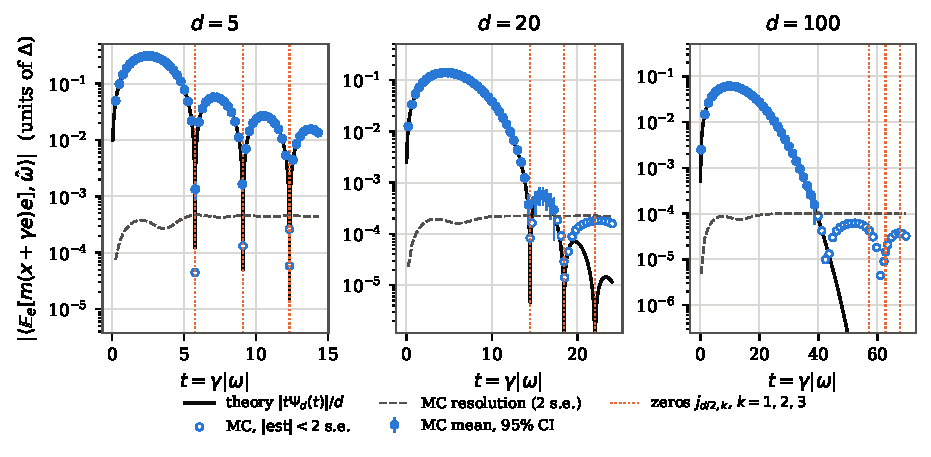
\includegraphics[width=\textwidth]{figs/e1_1_bessel_sweep.pdf}
\caption{E1.1, компонента $\E_e[m(x+\gamma e)e]$ вдоль $\omega$ в зависимости от $t=\gamma|\omega|$, логарифмическая шкала. Чёрная линия: теория $|t\Psi_d(t)|/d$. Закрашенные маркеры: среднее МК по 5~зёрнам с 95-процентным ДИ; полые: оценки в пределах 2~стандартных ошибок от нуля; пунктир: разрешение МК. При $d=100$ сигнал опускается ниже разрешения МК уже при $t\approx40$, задолго до первого нуля $j_{50,1}=57.1$.}\label{fig:e11}
\end{figure}

\textbf{Результат.} (A)~По 60~значениям $t$ стандартизованное отклонение от теории удовлетворяет $\max|z|=0.64,\,1.87,\,1.24$ при $d=5,20,100$; ни одного $|z|>2$ ($z$ положительно коррелированы по $t$ из-за общих случайных чисел). (B)~В нулях: $p$-значения $\chi^2_d$ $\ge0.096,\,0.048,\,0.12$, отклонений на уровне 5\%: $0/15,\,1/15,\,0/15$; медиана отношения $\norm{\hat\E}/\sqrt{\sum{\rm se}_i^2}$ равна $0.92,\,0.96,\,1.00$~--- оценка находится ровно на уровне шума МК. Значение пилотного расчёта из~\S\ref{sec:known} ($d=5$, $2.3\cdot10^{-4}$ при погрешности $2.2\cdot10^{-4}$) воспроизведено. (C)~Настроенные суперпозиции: гипотеза «$\E[me]=0$» отвергается в $4\%,\,2\%,\,7\%$ из 100~тестов (номинально 5\%); расстроенный контроль: $100\%,\,93\%,\,11\%$. При $d=100$ медианная норма расстроенного сигнала равна $1.1\cdot10^{-8}$ при шуме МК $3.5\cdot10^{-4}$, так что МК там не имеет мощности; этот режим проверяется вместо этого 40-значной квадратурой (S3: тождество $\E[\sin(te_1)e_1]=t\Psi_d(t)/d$ выполнено с относительной точностью $<10^{-20}$ в точках $0.95j$, $j$, $1.05j$ для первых трёх нулей, $d=100$).
\textbf{Вывод.} Предсказание подтверждено, нормировка подтверждена. Наблюдение: в высокой размерности бесселева часть невидима для любого теста на основе выборок задолго до нулей~--- это важно для H6.

\subsection{E1.2: логистическая регрессия с негладким шумом, $\tau=1$}
\textbf{Постановка.} $\ell_2$-регуляризованная логистическая регрессия как в эксперименте проекта с округляющим оракулом для выпуклых задач (тот же генератор задачи) с $d=10$, $n=50$, $\lambda=10^{-2}$; экземпляр задачи $=$ зерно; область $B_R$, $R=2\norm{x_*}$ ($\approx8.3$--$9.2$); $M=\norm A_{\rm op}/\sqrt n+\lambda R\approx0.54$; $\gamma=0.05$; $\Delta_{\rm ref}=M\gamma/\sqrt d$.
Шум: состояние $s=(k,\sigma)$, где $k$~--- свежий 64-битный ключ, а $\sigma=\pm1$, разыгрываются независимо в каждом раунде; $\delta(x,s)=\sigma\Delta\,\eta(\mathrm{hash}(\mathrm{cell}(x),k))$, $\eta=\pm1$, кубические ячейки со стороной $\gamma/(2\sqrt d)$. Тогда $m\equiv0$ (в классе для всех радиусов), а два значения пары~--- независимые $\pm\Delta$: это самый негладкий допустимый шум.
Метод: алгоритм~1 с $t_0=0$, $N=300$, $\eta=0.5/L$, усреднение по хвосту~--- по последним $N/2$ итерациям (отклонение от теор.~\ref{thm:alg}, где усредняются все итерации; задача гладкая и сильно выпуклая, поэтому константы теоремы для липшицева класса не используются~--- эксперимент проверяет \emph{масштабирование}). Сетка: $\Delta\in\{0,1,10,100\}\Delta_{\rm ref}$, $B\in\{4^0,\dots,4^{b}\}$, $b=7,7,8,9$.
Контроль (вне класса): замороженное состояние ($\tau=\infty$), шум $10\Delta_{\rm ref}\,\mathrm{sign}\sin(\sqrt d\ip vx/\gamma+\varphi)$, смещение которого при фиксированном состоянии $\asymp\sqrt d\Delta/\gamma$ не может быть усреднено.
\textbf{Предсказание} (зафиксировано до исследования): цель достигается при всех $\Delta$, требуемый бюджет растёт как $\Delta^2$. До основного запуска сделано количественным: основная цель $\varepsilon=0.03$ ($\approx11\%$ от $f(0)-f^*$), $T_\varepsilon$ для каждого зерна по интерполяции в логарифмических осях, наклон на $\{10,100\}\Delta_{\rm ref}$ равен $2\pm0.3$.
\textbf{Опровержение.} Плато ошибки (floor), не зависящее от $T$ (как ожидается от контроля).
\textbf{Журнал отклонений.} Верхний конец сетки по $B$ для $100\Delta_{\rm ref}$ ($4^9$) был задан после пилотного замера времени (зерно~0, $B\le4096$, $10\Delta_{\rm ref}$), показавшего, что $\varepsilon=0.03$ не будет достигнуто при $B\le4^8$; $\varepsilon$ и предсказание не менялись. После основного запуска был добавлен тест совмещения без интерполяции E1.2b (ниже), поскольку оценка наклона зависит от интерполяции вблизи излома (knee) кривых.

\begin{figure}[h]\centering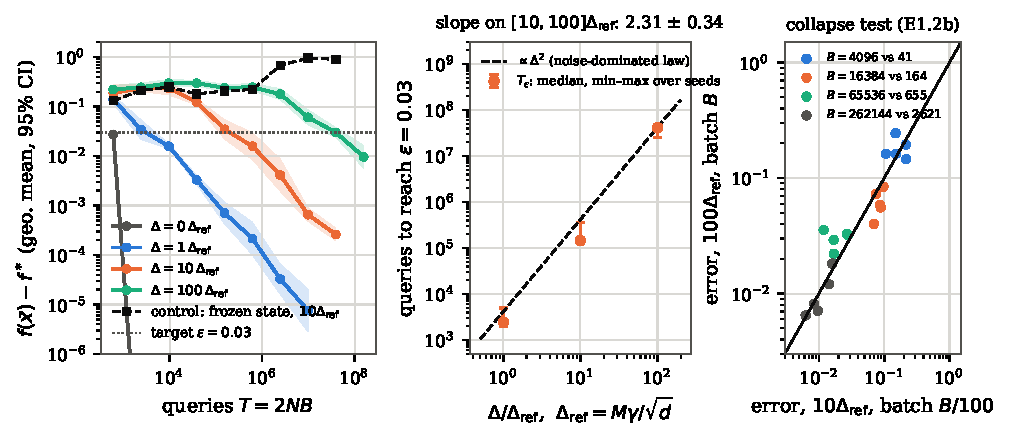
\includegraphics[width=\textwidth]{figs/e1_2_logistic.pdf}
\caption{E1.2. Слева: $f(\bar x)-f^*$ в зависимости от числа запросов $T=2NB$ (логарифмические оси), среднее геометрическое по 5~зёрнам с полосой 95-процентного ДИ; чёрный пунктир: контроль с замороженным состоянием. В центре: число запросов, нужное для достижения $\varepsilon=0.03$, в зависимости от $\Delta/\Delta_{\rm ref}$ (медиана, минимум--максимум по зёрнам), с законом $\Delta^2$, проведённым через точку $100\Delta_{\rm ref}$. Справа (E1.2b): ошибка при $100\Delta_{\rm ref}$ с пакетом $B$ против ошибки при $10\Delta_{\rm ref}$ с пакетом $B/100$, то же зерно; диагональ~--- точное масштабирование $\Delta^2$.}\label{fig:e12}
\end{figure}

\textbf{Результат.} Цель достигается для $5/5$ зёрен при каждом $\Delta$: медиана $T_\varepsilon=6.0\cdot10^2$ ($\Delta=0$, первая точка сетки), $2.4\cdot10^3$ ($1\Delta_{\rm ref}$, диапазон $1.9$--$5.0\cdot10^3$), $1.5\cdot10^5$ ($10\Delta_{\rm ref}$, $1.3$--$3.6\cdot10^5$), $4.2\cdot10^7$ ($100\Delta_{\rm ref}$, $2.5$--$4.6\cdot10^7$). При наибольшем пакете ошибка при $100\Delta_{\rm ref}$ всё ещё убывает (медиана $8.2\cdot10^{-3}$ при $T=1.6\cdot10^8$): плато нет. Наклон $\log T_\varepsilon$ по $\log\Delta$ на $[10,100]\Delta_{\rm ref}$ (попарно по зёрнам): $2.31\pm0.34$ (95-процентный ДИ $[1.97,2.65]$; по зёрнам $2.37,2.55,2.47,2.31,1.84$); чувствительность к цели: $2.16\pm0.27$ ($\varepsilon=0.02$), $2.11\pm0.33$ ($0.05$), $2.03\pm0.15$ ($0.1$).
\textbf{E1.2b (совмещение).} При согласованных пакетах ($B$ при $100\Delta_{\rm ref}$ против $B/100$ при $10\Delta_{\rm ref}$, 4~размера пакета $\times$ 5~зёрен) $\log_{10}(\mathrm{err}_{100}/\mathrm{err}_{10})=0.017\pm0.081$, т.\,е.\ отношение ошибок равно $1.04$ (95-процентный ДИ $[0.86,1.25]$): ошибка зависит от $(\Delta,B)$ только через $B/\Delta^2$ в пределах погрешности.
\textbf{Контроль.} Ошибка при замороженном состоянии не убывает с ростом $B$ (среднее геометрическое $0.13\to0.90$ от $B=1$ до $4^8$; наклон по последним четырём точкам $+0.33\pm0.59$): критерий опровержения обладает мощностью.
\textbf{Вывод.} Качественное предсказание подтверждено (цель достигается при каждом $\Delta$, плато нет). Заранее зафиксированный количественный критерий (наклон $2\pm0.3$ при $\varepsilon=0.03$) не выполнен с небольшим отрывом: точечная оценка $2.31$ на $0.01$ выше диапазона. Её ДИ $[1.97,2.65]$ содержит $2$, другие цели дают $2.03$--$2.16$, а тест совмещения без интерполяции даёт отношение $1.04$ $[0.86,1.25]$; поэтому мы сообщаем закон для бюджета как «согласующийся с $\Delta^2$», а не как выполненный заранее зафиксированный критерий. (H1.4b опирается на доказательство, а не на E1.2.)

\subsection{E1.3: настроенная волна при втором радиусе}
\textbf{Постановка.} $\gamma_1=\Delta=1$, $|\omega|=j_{d/2,k}$ ($k=1,2,3$), $d\in\{5,20,100\}$; 70~логарифмически равномерных отношений $\gamma_2/\gamma_1\in[0.05,3.2]$ плюс все отношения нулей в этом диапазоне и $\sqrt2$; $10^6$ направлений на зерно. Измеряемая величина~--- смещение двухточечной оценки при радиусе $\gamma_2$, $\beta=(d/\gamma_2)\E_e[m(x+\gamma_2e)e]$, вдоль $\hat\omega$ при $\sin=1$.
\textbf{Предсказание.} $\abs\beta=\Delta|\omega|\abs{\Psi_d(\gamma_2|\omega|)}$ (предл.~\ref{prop:quant}); нуль ровно при $\gamma_2/\gamma_1=j_{d/2,l}/j_{d/2,k}$, ненулевое значение при $\sqrt2$.
\textbf{Опровержение.} Отклонение от кривой сверх погрешности МК; обращение смещения в нуль при отношении общего положения.

\begin{figure}[h]\centering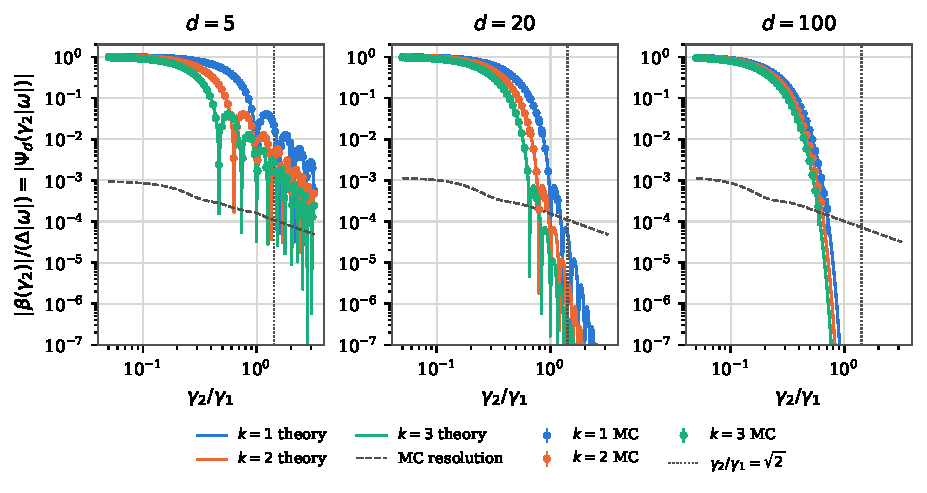
\includegraphics[width=\textwidth]{figs/e1_3_two_radii.pdf}
\caption{E1.3, нормированное смещение $|\beta(\gamma_2)|/(\Delta|\omega|)$ в зависимости от $\gamma_2/\gamma_1$ (логарифмические оси) для волн, настроенных на первые три нуля при $\gamma_1$. Линии: $|\Psi_d(\gamma_2|\omega|)|$; точки: МК (5~зёрен, 95-процентный ДИ), показаны там, где разрешены; пунктир: разрешение МК.}\label{fig:e13}
\end{figure}

\textbf{Результат.} По всем разрешённым и неразрешённым точкам $\max|z|=1.14,\,2.41,\,1.85$; доля $|z|>2$: $0\%,\,6.8\%,\,0\%$ из $276,\,309,\,315$ точек (коррелированы через общие случайные числа). При $\gamma_2=\sqrt2\gamma_1$, $d=5$: измерено $0.02232,\,0.00361,\,0.00270$ против теоретических $0.02231,\,0.00359,\,0.00270$ (стандартная ошибка $\le8.5\cdot10^{-5}$)~--- второй радиус общего положения обнаруживает волну. При $d=20,100$ теоретическое значение при $\sqrt2$ ($5\cdot10^{-5}$ и $3\cdot10^{-18}$) ниже разрешения МК. При $\gamma_2=0.1\gamma_1$ теоретическое смещение (за которым следует МК) лежит между $0.798\,\Delta|\omega|$ ($d=100$, $k=3$) и $0.976\,\Delta|\omega|$ ($d=5$, $k=1$), т.\,е.\ $\ge0.79\,\Delta|\omega|$ во всех девяти случаях (значения~--- в предл.~\ref{prop:quant} и в сохранённых результатах). Радиус половинного смещения: $|\Psi_d|=\frac12$ при $\gamma_2/\gamma_1=0.52,\,0.38,\,0.21$ ($d=5,20,100$), что согласуется с $\sqrt{2\ln2\,(d+2)}/j_{d/2,1}$.
\textbf{Вывод.} Предсказание подтверждено. Уточнение: второй радиус теоретически исключает настроенную волну, но на практике видит её с заметным смещением только \emph{меньший} радиус $\gamma_2\lesssim\gamma_1\sqrt{2(d+2)}/j_{d/2,1}$.

\subsection{E1.4 (новый): аддитивность $d$ и $\tau$ во втором моменте пакетной оценки}
\textbf{Постановка.} Шум $\delta(x,(k,\sigma))=\sigma\Delta\,\mathrm{sign}\sin(\sqrt d\ip{v_k}x/\gamma+\varphi_k)$, $K=512$ случайных $(v_k,\varphi_k)$, $\sigma=\pm1$ (так что $\E_\pi\delta\equiv0$: в классе для всех радиусов, максимальное смещение при фиксированном состоянии $\asymp\sqrt d\Delta/\gamma$). Ленивая цепь с перевыбором: с вероятностью $\alpha=1-1/\tau_{\rm nom}$ остаётся в текущем состоянии, иначе заново выбирает его из $\pi$; $\tau_{\rm nom}\in\{1,4,16,64,256\}$ ($\tmix=1,5,22,88,354$); $d\in\{10,40,160\}$; $f\equiv0$, $x=0$, $s_1\sim\pi$; $B=32\tmix+64$; 300~пакетов на зерно.
\textbf{Предсказание (точное, без свободных параметров).} $B\,\E\norm{\bar g}^2=A+S\,[1+2\sum_{t=1}^{B-1}(1-\frac tB)\alpha^t]$, где $S=\E_\pi\norm{b}^2$ и $A=\E\norm{n}^2-S$ вычисляются точными одномерными интегралами по распределению $e_1$ (неполная бета-функция); это следует из доказательства леммы~\ref{lem:var}(c) с точной автокорреляцией $\alpha^t$ ленивой цепи. Оценка: $(d+8\tmix-3)\,d\Delta^2/\gamma^2$.
\textbf{Опровержение.} Отклонения сверх объединённой погрешности МК; рост порядка $d\cdot\tau$.

\begin{figure}[h]\centering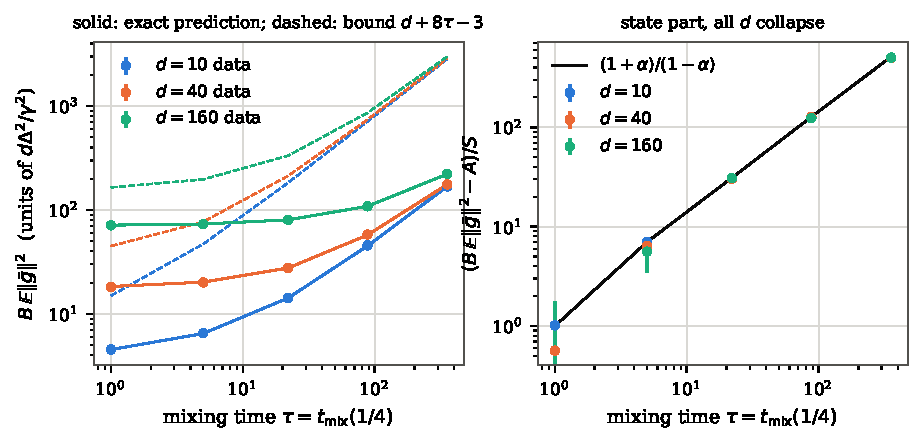
\includegraphics[width=0.95\textwidth]{figs/e1_4_batch_variance.pdf}
\caption{E1.4. Слева: $B\E\norm{\bar g}^2$ в единицах $d\Delta^2/\gamma^2$ в зависимости от $\tmix$ (логарифмические оси); сплошная линия: точное предсказание; пунктир: оценка леммы~\ref{lem:var}. Справа: зависящая от состояния часть $(B\E\norm{\bar g}^2-A)/S$; все размерности ложатся на $(1+\alpha)/(1-\alpha)$ (вариант для конечного $B$), наклон~1 по $\tau$.}\label{fig:e14}
\end{figure}

\textbf{Результат.} Во всех 15~ячейках относительное отклонение от точного предсказания $\le1.41\%$, объединённые $z\in[-1.19,1.55]$. Наклон зависящей от состояния части по $\tmix$ (логарифмические оси, $\tmix\ge5$): $1.003\pm0.025$, $1.02\pm0.05$, $1.05\pm0.11$ при $d=10,40,160$. Подобранные константы: $A/d^2=0.42$--$0.45$, $S/d=0.30$--$0.33$, так что $B\E\norm{\bar g}^2\approx(0.44\,d+0.43\,\tmix)\,d\Delta^2/\gamma^2$~--- аддитивно по $d$ и $\tau$ и $\le0.43$ от оценки.
\textbf{Вывод.} Предсказание подтверждено; константа $8$ в лемме~\ref{lem:var} для этой цепи завышена примерно в $20$ раз.

%=====================================================================================================
\section{Вердикт}\label{sec:verdict}
\begin{center}\small
\begin{tabularx}{\textwidth}{@{}p{5.2cm}p{3.0cm}X@{}}
\toprule
\textbf{Утверждение} & \textbf{Статус} & \textbf{На что опирается}\\\midrule
H1.1a $E_\pi$ и $E_e$ перестановочны & доказано при условии (совместная измеримость) & лемма~\ref{lem:fubini} \\
H1.1b $\frac d\gamma\E_e[\delta(x+\gamma e,s)e]=\nabla\hat\delta_\gamma$ & доказано: почти всюду для ограниченных борелевских; всюду в $\cG_\gamma$; вне его поточечно нарушается & лемма~\ref{lem:stokes}; V3 (гладкий и негладкий шум, $\max|z|\le1.7$), V7 \\
H1.1c (2) $\iff\hat m_\gamma\equiv c$; $\xi$ не ограничена & доказано & предл.~\ref{prop:reduction} \\
H1.1d выбор прочтения не влияет на результаты & доказано для всех результатов этого отчёта; для H3/H5~--- при условии, что их конструкции лежат в $\cG_\gamma$ & \S\ref{sec:theory}, «Какое прочтение» \\
H1.2a плоская волна допустима $\iff J_{d/2}(\gamma|\omega|)=0$; нормировка $\Delta t\Psi_d(t)/d$ & доказано; подтверждено численно & следствие~\ref{cor:waves}; E1.1; S2, S3 \\
H1.2b полное описание через простые слои на сферах & доказано на $\R^d$ (ограниченные $m$, глобально); на $B_R$ класс шире, только примеры & теор.~\ref{thm:fourier}; S4, S6 \\
H1.3a все $\gamma\le\gamma_0$ (или $\gamma_n\to0$) $\Rightarrow m\equiv c$ & доказано (локально, на $B_R$) & теор.~\ref{thm:allgamma} \\
H1.3b достаточно двух радиусов с отношением $\notin Q_d$; результат точен & доказано на $\R^d$ для ограниченных измеримых $m$; на $B_R$ только процитировано (локальная теорема о двух радиусах) & теор.~\ref{thm:tworadii}; V8; E1.3 \\
H1.3c второй радиус $\gamma_2\gtrsim\gamma_1$ количественно слаб при большом $d$ & доказано для плоских волн (оценка), подтверждено численно & предл.~\ref{prop:quant}; E1.3 \\
\bottomrule
\end{tabularx}
\end{center}
\begin{center}\small
\begin{tabularx}{\textwidth}{@{}p{5.2cm}p{3.0cm}X@{}}
\toprule
\textbf{Утверждение} & \textbf{Статус} & \textbf{На что опирается}\\\midrule
H1.4a явный алгоритм, смещение $\le\varepsilon/(8R)$, второй момент $\le V/B$, $V\asymp dM^2+(d+\tau)d\Delta^2/\gamma^2$ & доказано & лемма~\ref{lem:var}; E1.4 (точно до $1.41\%$); V5, V6, V10 \\
H1.4b $T(\Delta)=O(\Delta^2)$ явно; $\Dmax=\infty$ без бюджета и при «полиномиальном числе вызовов» & доказано при условии: класс всех радиусов (безусловно) или класс с фиксированным радиусом при $\gamma\le\varepsilon/(4M)$; вариант «в среднем», вариант «по вероятности» с заменой $\varepsilon\to\beta\varepsilon$ & теор.~\ref{thm:alg}, следствия~\ref{cor:degenerate}, \ref{cor:prob}; V9; E1.2 \\
H1.4c $\Dmax(T)\gtrsim\frac{\varepsilon\gamma}R\sqrt{T/(d(d+\tau))}$ (первая ветвь нижней половины H2) & доказано при условиях: $\gamma\le\varepsilon/(4M)$, $T\ge2T_1(\Delta)$ (так что $T\gtrsim\tau(MR/\varepsilon)^2\log$, не режим $\tau\gtrsim T$), с точностью до $\log$ в $t_0$ и констант; вариант «в среднем», вариант «по вероятности» с заменой $\varepsilon\to\beta\varepsilon$ & следствия~\ref{cor:lower}, \ref{cor:prob}; замечание~\ref{rem:h2} \\
H1.5a бесплатные холостые раунды делают $\tau$ несущественным & доказано (вариант «по вероятности»; сравнение с классом независимых одинаково распределённых состояний) & предл.~\ref{prop:wait} \\
H1.5b $q=1$ и $q=2$: та же вырожденность & доказано & предл.~\ref{prop:q1}; V10 \\
H1.5c $\Dcp(C)\ge M\gamma/\sqrt{2d+8\tau-3}$ (ожидаемая картина, нижняя сторона) & доказано при $C\ge\frac{149}4(6+t_0/d)$ и $\gamma\le\varepsilon/(4M)$, вариант «в среднем» ($C=261$, если $\tau\lceil\log_2(16MR/\varepsilon)\rceil\le d$); вариант «по вероятности» с заменой $\varepsilon\to\beta\varepsilon$, $C\to C/\beta^2$ & следствия~\ref{cor:cp}, \ref{cor:prob} \\
H1.5d $\Dcp(C)\lesssim M\gamma/\sqrt d$ (верхняя сторона) & остаётся гипотезой (H3.2) & --- \\
\bottomrule
\end{tabularx}
\end{center}

%=====================================================================================================
\section{Следствия}\label{sec:contrib}
\subsection{Для общей задачи}
\begin{enumerate}
\item Без бюджета порог вырождается: $\Dmax=\infty$ в классе всех радиусов (безусловно) и в классе с фиксированным радиусом при $\gamma\le\varepsilon/(4M)$, в том числе при «полиномиальном числе вызовов» (следствие~\ref{cor:degenerate}; доказано при этих условиях, вариант «в среднем», вариант «по вероятности»~--- по следствию~\ref{cor:prob}). Поэтому невырожденный порог~--- это \emph{функция} $\Dmax(T)$ от бюджета раундов при протоколе, зафиксированном как в опр.~\ref{def:dmax}.
\item «Ожидаемая картина»~--- это утверждение о $\Dcp(C)=\Dmax(C\,T_0)$; её нижняя сторона доказана при $\gamma\le\varepsilon/(4M)$ и $C\ge\frac{149}4(6+t_0/d)$ в варианте «в среднем» (следствие~\ref{cor:cp}; вариант «по вероятности»~--- по следствию~\ref{cor:prob}); верхняя сторона остаётся гипотезой (H3.2).
\item Класс: (2) для всех радиусов из $(0,\gamma_0]$ равносильно $\E_\pi\delta(x,\cdot)={\rm const}$ для почти всех $x$ (теор.~\ref{thm:allgamma}, доказано). В этом классе $\gamma$ не входит в определение класса и является параметром алгоритма; класс с фиксированным радиусом содержит бесселевы волны (теор.~\ref{thm:fourier}, доказано), влияние которых на другие радиусы~--- предмет H6.
\item Равномерная геометрическая эргодичность входит только через $d(t)\le2^{-\lfloor t/\tau\rfloor}$ (лемма~\ref{lem:var}); для общего пространства состояний это \emph{и есть} равномерная эргодичность, так что H1 не ослабляет это предположение постановки задачи; его ослабление~--- предмет H9.
\item Округление с равномерным сдвигом удовлетворяет (2) для всех радиусов ($\E_c\delta$~--- среднее «пилы» округления за период, константа), т.\,е.\ лежит в классе всех радиусов с $m\equiv{\rm const}$. Но цепь округления порождается методом, что опр.~\ref{def:dmax} исключает; округление попадает в $\cN$ только после расширения H8.
\end{enumerate}

\subsection{Для других гипотез}
H2: \emph{первая ветвь} её нижней половины ($\gtrsim\frac{\varepsilon\gamma}R\sqrt{T/(d(d+\tau))}$) доказана с точностью до логарифма прогрева при $\gamma\le\varepsilon/(4M)$ и $T\ge2T_1(\Delta)$, т.\,е.\ в режиме $T\gtrsim\tau(MR/\varepsilon)^2\log(R\sqrt d\Delta/(\gamma\varepsilon))$, в варианте «в среднем» (следствие~\ref{cor:lower}). Не охвачены: режим $\tau\gtrsim T$, вторая ветвь $\frac{\varepsilon\gamma}R\sqrt{\ln T/d}$ (замечание~\ref{rem:h2}: без $\sqrt{\ln T}$ и при $T\ge J(2K+1)$ она может следовать из arXiv:2306.16371v5, предл.~IV.1, не перепроверено) и вся верхняя половина.
H4: дисперсионная часть сведения к Prokhorov et al.\ выполнена напрямую (лемма~\ref{lem:var}); для H4 остаются устранение логарифма прогрева и гарантии для последней итерации.
H3: постановка теперь зафиксирована (опр.~\ref{def:dmax}); верхняя оценка $\Dcp\lesssim M\gamma/\sqrt d$~--- это в точности H3.2.
H5.1: согласуется («повтори и усредни»~--- ещё один путь к $\Dmax=\infty$).
H6: поддержана. Её механизм~--- при $\gamma>\gamma_\varepsilon$ метод должен использовать меньший радиус, где бесселева часть $m$ действует как систематическая ошибка величины $\approx\Delta d/(2\gamma)$,~--- подтверждён предл.~\ref{prop:quant} и E1.3 (смещение $\ge0.79$--$0.98\,\Delta|\omega|$ при $\gamma_2=0.1\gamma_1$). Этот отчёт добавляет для H6 лишь соображение об экспериментах, в которых меняется радиус: для таких экспериментов диапазон $\gamma'>\gamma$ неинформативен при $d\ge20$ (смещение $\le7.5\cdot10^{-4}\,\Delta|\omega|$, ниже разрешения Монте-Карло). В рекомендуемом классе всех радиусов H6 не возникает.
H8, H9: предположение об экзогенной цепи и использование равномерного перемешивания теперь сформулированы явно; это два места, которые предстоит ослабить.

\subsection{Открытые вопросы}
\begin{itemize}
\item Верхняя сторона уровня, сохраняющего сложность, $\Dcp(C)\lesssim M\gamma/\sqrt d$ для двухточечных методов радиуса $\gamma$ (H3.2); для произвольных точек запроса она может быть неверна (H3.3).
\item Вторая ветвь $\frac{\varepsilon\gamma}R\sqrt{\ln T/d}$ нижней половины H2 и режим $\tau\gtrsim T$ (замечание~\ref{rem:h2}).
\item Класс с фиксированным радиусом при $\gamma>\varepsilon/(4M)$, где $\Dmax$ без бюджета может быть конечным (следствие~\ref{cor:degenerate}(iv); H6).
\item Теорема о двух радиусах на шаре $B_R$ (здесь только процитирована) и класс с фиксированным радиусом на $B_R$, который шире, чем на $\R^d$ (теор.~\ref{thm:fourier} и абзац об области применимости после неё).
\item Модельные решения, от которых зависит $\Dmax$: учитываются ли холостые раунды (если они бесплатны, $\tau$ выпадает, предл.~\ref{prop:wait}), произвольны ли $q$ точек одного состояния или это только $x\pm\gamma e$ ($\Dmax$ или $\Dmax^{2\rm pt,\gamma}$), и требуется ли (2) на одном радиусе или на всех радиусах $\le\gamma_0$. Опр.~\ref{def:dmax} фиксирует один выбор; в~\S\ref{sec:theory} (H1.5) указано, как влияют остальные.
\item Цепь, порождённая методом (H8), и предположения о перемешивании слабее равномерной эргодичности (H9).
\end{itemize}

\subsection{Границы новизны}
Постановка задачи уже говорит о «полиномиальном числе вызовов», а схема MALN из работы Pasechnyuk-Vilensky et al.\ (arXiv:2306.16371v5, опр.~II.2) уже содержит $T$; если объектом задачи изначально подразумевался уровень, сохраняющий сложность, то определительная часть H1~--- это уточнение, а не новый результат. Новым в любом случае является: структурная теорема для класса (теор.~\ref{thm:fourier}--\ref{thm:tworadii}, предл.~\ref{prop:quant}), явная формула бюджета с аддитивным $d+\tau$ и её следствие~--- первая ветвь нижней половины H2 в режиме $T\gtrsim\tau(MR/\varepsilon)^2\log$,~--- а также чувствительность к протоколу (предл.~\ref{prop:wait}).

%=====================================================================================================
\appendix
\section{Проверки}\label{app:checks}
\begin{center}\small
\begin{tabularx}{\textwidth}{@{}lXl@{}}
\toprule
\textbf{ID} & \textbf{Проверка} & \textbf{Результат}\\\midrule
V1 & $\Psi_d(t)=\E_u\cos(tu_1)$, квадратура, $d\in\{2,3,5,20\}$ & ошибка $6\cdot10^{-15}$ \\
V2 & $\Phi_d'=-(t/d)\Psi_d$, конечные разности, $d\le100$ & ошибка $1.4\cdot10^{-9}$ \\
V3 & формула Стокса на шаре: МК-интеграл по сфере против конечных разностей среднего по шару ($d=5$; гладкие волны и хэш-шум по сетке) & $\max|z|=1.2$ (гладкий), $1.7$ (негладкий); против точного $1.6$ \\
V4 & $\E|e_1|\le1/\sqrt d$; смещение в худшем случае $\le\sqrt d\Delta/\gamma$ & пройдена \\
V5 & $\E\norm{g_f}^2\le d^2M^2/(d-1)$ для четырёх тестовых функций, $d\in\{2,5,20\}$ & макс.\ отношение $0.95$ \\
V6 & $\sum_{t\ge1}2^{-\lfloor t/\tau\rfloor}=2\tau-1$; $d(\ell\tmix)\le2^{-\ell}$; $\sum d(t)\le2\tmix-1$ (ленивые цепи) & пройдена \\
V7 & поточечное нарушение вне $\cG_\gamma$ (лемма~\ref{lem:stokes}(c)) & $S_g(0)_1=1.875=5\E|e_1|$, $0$ в остальных точках \\
V8 & $\sqrt2,1.5,\pi/2\notin Q_5$; расстояние до $Q_5$ убывает с ростом числа нулей & пройдена \\
V9 & формула~\eqref{eq:T}: наклон $\log T$ по $\log\Delta$ & $2.000$ \\
V10 & алгоритм~1 несмещён при ленивой цепи, $q=2$ и $q=1$ & $\max|z|=1.6,\ 2.7$ ($d$ компонент) \\
S1 & $(t^{-\nu}J_\nu)'=-t^{-\nu}J_{\nu+1}$, $\Phi_d'=-(t/d)\Psi_d$ (sympy, общее $d$) & точно \\
S2 & $\Psi_1,\Psi_3$ точно; $\Psi_2,\Psi_5$ до 50~знаков & точно / $3\cdot10^{-51}$ \\
S3 & тождество для плоской волны при $d=100$ вблизи нулей, 40~знаков & отн.\ ошибка $<10^{-20}$ \\
S4 & простые нули, $J_{d/2+1}(j_{d/2,k})\neq0$ & пройдена \\
S5 & константы $145/64$, $145/4$; блочная сумма & точно \\
S6 & $\rho\,\delta'(\rho)=-\delta(\rho)$ & точно \\
S7 & формула $\E|e_1|\le1/\sqrt d$, $d=2..200$ & пройдена \\
\bottomrule
\end{tabularx}
\end{center}
V1--V10~--- численные проверки (numpy/scipy); S1--S7~--- символьные проверки и проверки с высокой точностью (sympy/mpmath). Все запуски вместе занимают $\approx35$~мин на 2~ядрах CPU (основное время занимает E1.2). Рисунки строятся только по сохранённым сырым результатам.

\paragraph{Что не проверялось.} Локальная теорема о двух радиусах на шаре и литература о задаче Помпейю для общего $d$ (только цитируются); номер теоремы в обзоре arXiv:2211.13566; результаты Prokhorov et al.\ (в доказательствах не используются); эксперименты с $\tau>1$ на задаче оптимизации (E1.4 проверяет оценку градиента, а не метод целиком); размерности выше $d=10$ в E1.2 (вычислительная стоимость на CPU).

\paragraph{История редакций.} Отчёт был исправлен после независимой рецензии (10~ноября 2026~г.) и отредактирован для публикации (11~ноября 2026~г.); редактирование для публикации не изменило ни одного утверждения, доказательства, статуса или числа.

\end{document}
